\cotefile{150}
\scanpage{44}
\unsure{précisément}, \unsure{on a} de plus une application croiss. et continue
\[
(2^\circ)\quad (25)\qquad \Sigma_*\longrightarrow I
\]
(d'où
\[
\Sigma_*=\coprod_{i\in I}\Sigma_i\ ,\quad
\Sigma_{**}=\underset{i\leq j}{\deleted{\sum}\inserted{\coprod}}\Sigma_{ij})
\]
\deleted{\unsure{avec} $\Sigma_{ii}\simeq\Sigma_i$)}

Et on \deleted{\unsure{demande}} suppose que $\forall i,j$, \inserted{$i\leq j$} le morphisme but
\[
\Sigma_{ij}\longrightarrow\Sigma_j
\]
est un \deleted{\unsure{immersement}} plongement fermé \inserted{``cylindrique''}, (-- ce qui implique (par injectivité) que (25\unsure{$^*$|$^\circ$}) a la propriété que si $z\in\Sigma_*$ est au dessus de $j$ et si $i\leq j$, alors il existe \uline{au plus} un $y\in\Sigma_*$ \deleted{au} dessous de $i$, avec $y\leq z$.
\margin{Condition \unsure{\textcircled{a}}}
\margin{\unsure{via} $\Sigma_*^{\leq 2}\longrightarrow I^{\leq 2}$ \unsure{injectif}}

Cela implique aussi
\[
(26)\qquad\Sigma_{ii}=\Sigma_i
\]
\deleted{On suppose de plus que pour $z\in$ $\unsure{i}\leq j\leq k$, $\unsure{\Sigma_i}$}
\margin{\deleted{condition \unsure{b)}}}
\[
(27)\qquad \uline{\Sigma(n)}=\text{ens des drapeaux stricts de longueur }n\text{ de }\Sigma
\]
ou
\[
(27)\qquad
\begin{aligned}
\Sigma(n)&\longrightarrow\deleted{\unsure{I}}\operatorname{Drap}_n(I)\quad\text{(drapeaux stricts)}\\
\Vert\quad&\\[-1ex]
\coprod_{\substack{(i_0<\unsure{\cdots}<i_n)\text{ drapeau strict en}\\ I\text{ de longueur }n}}\Sigma_{i_0- i_n}&
\end{aligned}
\]
\margin{OK}
\margin{\unsure{permet ainsi l'énoncé de la condition (\unsure{b})}}
\mspage{43}

\scanpage{45}
\mspage{18}
On suppose, pour $i<j<k$
\[
(28)\qquad\Sigma_{ijk}=\Sigma_{ik}\cap\Sigma_{jk}\qquad
(\text{a priori }\Sigma_{ijk}\subset\Sigma_{ik}\cap\Sigma_{jk})
\]
\margin{Condition \textcircled{b}}
ce qui signifie aussi que $\forall z\in\Sigma_*$ au dessus d'un $k\in I$ (i.e. $z\in\Sigma_k$), l'hom. d'ens.
\[
\Sigma_*\longrightarrow I
\]
(\inserted{\unsure{qui par $1^\circ$}} induit une application
\[
\Sigma_{*\unsure{\leq}z}\unsure{\hookrightarrow|\longleftrightarrow} I_{\leq k}
\]
) induit
\[
(29)\qquad (\Sigma_*)_{\leq z}\unsure{\hookrightarrow|\longleftrightarrow} I_{\leq k}
\]
\margin{l'ordre de $(\Sigma_*)_z$ est \uline{induit} par celui de $I_{\leq k}$}
\margin{Ceci implique que si $d,d'$ sont des \unsure{drap.}\inserted{drapeaux} tels que $d''=d\cup d'$ soit un drapeau et que $d,d'$ \unsure{ay. même} élément final $i$, i.e. $d,d'$ aient \unsure{$=$} \uline{\unsure{l'injection|l'égalité}} alors $\Sigma_{d''}=\Sigma_d\cap\Sigma_{d'}$ dans $\Sigma_i$.}

On suppose de plus que si $i,j\leq k$ n'ont pas de minorant \inserted{dans $I$}, alors
\[
\Sigma_{ik}\cap\Sigma_{jk}=\varnothing
\]
(si $i,j$ ont un minorant $l$, alors
\[
\Sigma_{ik}\cap\Sigma_{jk}\subset\ )
\]
\margin{Condition \textcircled{c} \unsure{Gros}}
\margin{Implique que si $d,d'$ sont deux drapeaux ayant final $k$, et si $d\cup d'$ n'est pas un drapeau, alors $\Sigma_d\cap\Sigma_{d'}=\varnothing$.}
\margin{\textcircled{b} et \textcircled{c} impliquent que si $(d_\alpha)_{\alpha\in\unsure{A}}$ est une famille \inserted{\unsure{finie}} de drapeaux de $I$, \deleted{\unsure{$\forall\alpha$}} \unsure{$\forall\alpha\in A$} \unsure{aient|sont} final $k$, donc les $\Sigma_{d_\alpha}\subset\Sigma_k$, alors $\bigcap\Sigma_{d_\alpha}$ est \uline{vide} si $\bigcup d_\alpha$ n'est pas un drapeau, et $=\Sigma_{\cup d_\alpha}$ sinon.}

On suppose enfin que le système des $\Sigma_{ik}$ (pour $k$ fixé, \inserted{$i\in I_{<k}$}), qui sont des sous-espaces \deleted{bord} \unsure{bord-ts} de $\Sigma_k$, sont \uline{transversaux}, ce qui signifie (grâce : \unsure{(30)}\inserted{et 28,}) que si on a un drapeau $d=(i_0,\!\ldots\!i_n,k)$, alors les $\Sigma_{i_0k},\Sigma_{i_1k}\ \ldots\ \Sigma_{i_n,k}$ dans $\Sigma_k$ sont des sous-ens \unsure{bordants} qui se coupent \uline{transversalement} le long de $\Sigma_d=\Sigma_{i_0- i_n,k}$.
\margin{Condition \textcircled{d}}
\margin{implique le $=$ dans les $\Sigma_d$, \unsure{on prend} les $\Sigma_{d'}\subset\Sigma_d$ (i.e. but pour $d'\supsetneqq d$, et \unsure{$l_i$} bord.\inserted{$d'=d\cup\{i\}$} \unsure{qui sont} toutes pour un drapeau de $d'$) dans $\Sigma_d$ \unsure{lisses}.}
\mspage{44}

\scanpage{46}
Enfin, dans le cas équisingulier on suppose que les
\[
\Sigma_{ij}\longrightarrow\Sigma_i
\]
sont des \uline{fibrations} (i.e. $\Sigma_{**}\xrightarrow{s}\Sigma_*$ est une fibration), et dans le cas des strates \unsure{non-singulières} on suppose que les $\Sigma_i$ sont des variétés à bord (i.e. $\Sigma_*$ variété à bord) -- ce qui implique que les $\Sigma_{ji}$ (\deleted{$j<i$} \unsure{tq-précédemment}) sont des sous-variétés à bord du \deleted{$\Sigma_i$} bord $\dot\Sigma_i$ de $\Sigma_i$, et les $\Sigma_{ji}$ ($j<i$ \inserted{\unsure{$i$ elt final}}) définissent (\inserted{\unsure{en dépit la cond$^{\mathrm n}$ d')} }) une stratification cylindrique du \deleted{$\unsure{\Sigma_*}$} bord par des variétés à bord -- Alors les $\Sigma_d=\Sigma_{i_1\ldots i_n}$ sont alors des variétés à bord \unsure{p.} et les $\Sigma_{d'}$ ($d'\supsetneqq d$, $d$ cofinal dans $d'$) \deleted{\unsure{en forment}} forment une stratification cylindrique du bord \deleted{de $\dot\Sigma_d$} de $\Sigma_*$.
\margin{condition e) ``équisingularité''}
\margin{Cela implique que $\Sigma_d\longrightarrow\Sigma_{d'}$ est une fibration, si $d'\subset d$ est un \uline{segment initial} de $d$.}
\margin{Condition f) ``non-singularité''}
\margin{$*$ cet ens d'indices des $d'$ s'identifie au sous-ens de
$\inserted{\widehat{\operatorname{Drap}}(I_{\cdot<i_1})\times}\widehat{\operatorname{Drap}}(I_{i_1<\cdot<i_2})\times\widehat{\operatorname{Drap}}(I_{i_2<\cdot<i_3})\times\ldots\times\unsure{\widehat{\operatorname{Drap}}(I_{i_{n-1}<\cdot<i_n})}$
où $\widehat{\operatorname{Drap}}$ désigne les drapeaux, \unsure{y.c. vides}, privé du \deleted{\unsure{drapeau}} pt unique \unsure{correspondant aux} drapeaux vides (pour $d'=d=(i_1,\ldots i_n)$).}
\margin{il s'identifie aussi à $\operatorname{Drap}(I_{<i_1}\coprod I_{i_1<\cdot<i_2}\coprod\ldots\coprod I_{i_{n-1}<\cdot<i_n})$}

Dans le cas d'équisingularité non-singulière, on suppose, en plus de e) et f), que les fibres des \inserted{fibrations} $\Sigma_{ij}\longrightarrow\Sigma_i$ sont des variétés à bord -- le \deleted{\unsure{réunion}} \inserted{fibré sur $\Sigma_i$} des bords des fibres est \deleted{formé des}\inserted{\unsure{réunion}} stratifié par les $\Sigma_d$, où $d$ \deleted{\unsure{donne}} parcourt les drapeaux qui contiennent \uline{strictement} \deleted{$\unsure{\Sigma}$} $(i,j)$ et ont $i$ comme premier
\deleted{\unsure{élément par l'ancien produit} $\widehat{\operatorname{Drap}}(I_{i<\cdot<j})\times\widehat{\operatorname{Drap}}(I_{>j})$}
\margin{Condition g)}
\margin{\unsure{drapeaux} \unsure{\deleted{côt. vide}}\qquad\unsure{drapeaux}\unsure{\deleted{stricts}}}
\mspage{45}

\scanpage{47}
\mspage{19}
\deleted{\uline{privé} de $(\varnothing,\varnothing)$ (qui corresp. au drapeau $i,j$ lui $\unsure{=}$ -- si on ne l'excluait pas, on aurait une stratification de $\Sigma_{(i,j)}$ lui-\unsure{mê}, non de son bord. Pour que $\Sigma_{ij}-\Sigma_i$ soit \inserted{(top.\unsure{C$^\infty$})} lisse, il f. et s. donc que $j$ soit un successeur de $i$, et que $j$ soit maximal dans $I$}
élément (pour être fibré sur $\Sigma_i$) et $j$ comme dernier (pour être contenu ds $\Sigma_{ij}$) s'\unsure{ident} donc \inserted{$\simeq$} $\operatorname{Drap}(I_{i<\cdot<j})$. Il est vide ssi $j$ est un successeur de $i$, qui est donc la condition pour que $\Sigma_{ij}-\Sigma_i$ soit lisse.

Plus généralement, si $d\subsetneqq d'$ est un segment initial, la fibration $\Sigma_{d'}\longrightarrow\Sigma_d$ est à fibres des variétés à bord, et le fibré des bords est stratifié cylindriquement par les $\Sigma_{d''}$ où $d''\supsetneqq d'$ (pour que $\Sigma_{d''}\overset{\unsure{\alpha}}{\hookrightarrow}\Sigma_{d'}$) est tel que $d'$ soit cofinal dans $d''$ (pour que $\Sigma_{d''}\hookrightarrow\Sigma_{d'}$) et que $d$ soit segment initial dans $d''$ (pour que $\Sigma_{d''}\longrightarrow\Sigma_{d'}$ soit \unsure{fibrant}) i.e. \deleted{\unsure{si on est le}} \inserted{si $d'=(i_1- i_n)$}, $d=(i_1,-i_p)$, \deleted{\unsure{alors $d''$ est de la forme}} $d'=d\coprod d'_0$ \deleted{plus grand élément de $d_p$ et plus grand élément} avec $d'_0=(i_{p+1},i_{p+2}\ldots i_n)$, alors les $d''$ correspondent aux
\deleted{\unsure{par $d'$} (donc $\alpha\leq\beta$), ce sont les drapeaux où $\beta$ comme plus grand élément, et \unsure{formé d'indices} \unsure{forme} $d\coprod d''_0$, où $d''_0\subset I_{\cdot>\alpha}$}
\inserted{\unsure{les} drapeaux \deleted{\unsure{finis}} $d''_0\subset I_{\cdot>i_p}$}, contenant \deleted{\unsure{les}} strictement $d'_0$ et tels que $d'_0$ soit cofinal dans $d''_0$, \deleted{\unsure{c'est donc un}} \inserted{l'un de ces $d''_0$, ou l'ens des $d''_0$, est en} corresp. biunivoque avec
\[
\operatorname{Drap}\bigl(I_{i_p<\cdot<i_{p+1}}\deleted{\unsure{\}}}\coprod I_{i_{p+1}<\cdot<i_{p+2}}\coprod\ldots\coprod I_{i_{n-1}<\cdot<i_n}\bigr)
\]
\mspage{46}

\scanpage{48}
On a lissité (à tous les coups) ssi \deleted{\unsure{pour}} la suite $i_p\ i_{p+1}\ldots i_n$ (à partir de $i_p$, pas de $i_1$ !) est \unsure{saturée}, i.e. chaque terme \inserted{(sauf le premier)} est successeur \inserted{dans $I$} du précédent.

11. \uline{Digression : où on laisse tomber} $I$.

Soit donné un ens. ordonné topologique, i.e. un \deleted{espace topologique} ens. ordonné $\Sigma=\Sigma(0),\Sigma(1)$, où $\Sigma(0)$ est un espace topologique, $\Sigma(1)$ une partie fermée de $\Sigma(0)\times\Sigma(0)$, qui soit le graphe d'une relation d'ordre. On suppose
\margin{\unsure{On retient ce cas}}

\textcircled{a}\quad $\Sigma(1)\xrightarrow{\mathrm{but}}\Sigma(0)$ est une immersion localement bordante, et propre (donc finie)

\deleted{\textcircled{b}} Cela implique que $\Sigma(0)\xrightarrow{\mathrm{diag}}\Sigma(1)$ est un isomorphisme sur une partie ouverte et fermée. Soit $\Sigma^{<}(1)$ le complémentaire de l'image, où l'on a une des inégalités strictes $i<j$. On désigne par $\Sigma^{<}(n)$ l'espace des drapeaux \uline{stricts} $i_0<i_1\ldots<i_n$ de longueur $n$. Les $\Sigma^{\unsure{*|<}}(n)$ \deleted{\unsure{sont forment|forment}} un espace \inserted{pré}\unsure{semi}-simplicial (\uline{NB} pas d'applications de dégénérescence, \deleted{\unsure{car par}} ils sont dans les $\Sigma(n)\ldots$). \deleted{Les} Si on a un
\mspage{47}

\scanpage{49}
\mspage{20}
diagramme d'inclusions \inserted{(croissantes)} d'ens tot. ordonnés
\[
(31)
\]
\diagram{\begin{tikzcd}[row sep=large,column sep=large]
&d''=d\cup d'&\\
d\arrow[ur,hook,no head]&&d'\arrow[ul,hook',no head]\\
&\delta=d\cap d'\arrow[ul,hook',no head]\arrow[ur,hook,no head]&
\end{tikzcd}}
tel que ce soit un diagramme cocart. dans la cat. des ens. ordonnés (p.ex $\delta$ segment initial de $d$, et $d'$ contenant l'élément final de $d$) alors le diagramme correspondant
\[
(32)
\]
\diagram{\begin{tikzcd}[row sep=large,column sep=large]
&\Sigma^{\unsure{<}}(d'')\arrow[dl]\arrow[dr]&\\
\Sigma^{<}(d)\arrow[dr]&&\Sigma^{<}(d')\arrow[dl]\\
&\Sigma^{\unsure{<}}(\delta)&
\end{tikzcd}}
est cartésien. \deleted{\unsure{(pour cela le cas est}}

Les conditions b c d du n\textsuperscript{o} précédent deviennent ici une seule (du type d)

\textcircled{b} Considérons un ens \deleted{\unsure{ens tot}} ordonné \inserted{de ``dim'' $\geq1$}, $d=(i_0,-i_n)$, et considérons le diagramme
\diagram{\begin{tikzcd}
\deleted{\unsure{\Sigma(n)}}\arrow[r,phantom,"\deleted{\longrightarrow}" description]&\deleted{\Sigma(0)}
\end{tikzcd}}
\[
(33)
\]
\diagram{\begin{tikzcd}[row sep=large,column sep=large]
&\Sigma^{<}(i_0,i_n)\arrow[dr,"\varphi_0"]&\\
\Sigma^{<}(d)\arrow[ur]\arrow[r]\arrow[ddr,bend right=15]&\Sigma^{<}(i_1,i_n)\arrow[r,"\varphi_1"]&\Sigma^{<}(i_n)\\
&\vdots&\\
&\Sigma^{<}(i_{n-1},i_n)\arrow[uur,"\varphi_{n-1}"']&
\end{tikzcd}}
\deleted{de \unsure{plongements} bordants.} d'immersions, où les $\varphi_0,\varphi_1,\ldots\varphi_n$ sont bordantes. On suppose
\margin{Plus précisément nous voulons que pour $x\in\Sigma^{\unsure{<}}(0)$, les $z_\alpha\in\Sigma^{<}(1)$ au dessus de $x$ (par but) sont en \uline{corr. biunivoque} avec les germes $B_\alpha$ des sous-ens. bord-ts, images locales des $\Sigma^{<}(1)$ en $z_\alpha$, que ces germes sont transversaux, et que les points \inserted{de $\Sigma^{\unsure{<}}(1)$} \deleted{\illegible{3}} \unsure{au dessus de $x$} \unsure{correspondants} \unsure{distincts} \unsure{déterminent} un drapeau \unsure{dans} \unsure{les $z_\alpha$}.}
\mspage{48}

\scanpage{50}
que \deleted{la famille soit}\inserted{au voisinage} de chaque pt de $\Sigma^{<}(d)\simeq\Sigma^{<}(n)$ $\Sigma^{<}(d)$ soit l'intersection \inserted{dans $\Sigma^{<}(i_n)\simeq\Sigma(0)$} des $\Sigma^{<}(\{i_\alpha,i_n\})_\alpha$ ($\simeq\Sigma^{<}(1)$), et que cette famille soit transversale.

Cela implique la chose analogue pour tout morphisme d'immersion
\[
\Sigma^{<}(d')\longrightarrow\Sigma^{<}(d)
\]
\margin{$d\subset d'$, $d,d'$ cofinaux (ont \unsure{le même} plus grand élément)}
\deleted{\unsure{dans} la structure,}
on considère les $d''$ entre $d$ et $d'$ (donc cofinaux avec $d$) qui sont de la forme $d\cup\{i\}$ ($i\in d'\smallsetminus d$) on regarde le diagramme
\[
(34)
\]
\diagram{\begin{tikzcd}[row sep=large,column sep=large]
&\Sigma^{<}(d\unsure{'}\cup j_0)\arrow[dr,"\text{bordant}"]&\\
\Sigma^{<}(d')\arrow[ur]\arrow[ddr,no head]&&\Sigma^{\unsure{*|<}}(d)\\
&\vdots&\\
&\Sigma^{<}(d\cup j_p)\arrow[uur,no head,"\text{bordant}"']&
\end{tikzcd}}
qui généralise (33), et on \deleted{suppose}\inserted{voit} qu'il satisfait la même condition de transversalité. Car on identifie tous les espaces envisagés, au voisinage des pts en jeu, à des sous-espaces de $\Sigma^{<}(\{\unsure{\alpha}\})\simeq\Sigma^{\unsure{*|<}}(0)$, décrits \inserted{(grâce à b)} comme des intersections partielles des certains sous-espaces bordants de $\Sigma^{<}(\{\unsure{\alpha}\})$, se coupant transversalement\ldots
\mspage{49}

\scanpage{51}
\mspage{21}
Il y a de plus des ``conditions de circonstance'' :

\textcircled{c} L'application $\Sigma^{<}(1)\xrightarrow{\mathrm{source}}\Sigma^{<}(0)$ est \inserted{propre et} fibrante (``condition \inserted{d'}isotrivialité''), cela implique que \deleted{\unsure{si}} si $d\subset d'$ est une inclusion d'ens finis tot. ordonnés, tel que $d$ soit segment initial de $d'$, alors $\Sigma^{\unsure{*|<}}(d')-\Sigma^{<}(d)$ est fibrante.

\textcircled{d} \deleted{Le} $\Sigma^{<}(0)$ est \deleted{\unsure{le}} une variété à bord, \uline{et} \inserted{$\Sigma^{<}(1)\xrightarrow{\mathrm{but}}\Sigma^{<}(0)$ a comme image son bord.} (``condition non singulière'') donc aussi les $\Sigma^{<}(d)$ (car un sous-espace bordant d'une variété à bord est une variété à bord \deleted{\unsure{qui doit}} \unsure{déterminer le bord}, de $=$ dim que celui-ci ?? \unsure{\}} ou on exige \deleted{\unsure{de plus la condition}} \inserted{que les $\Sigma^{<}(d)$ soient des} variétés à bord\ldots)
\margin{Dans tous les cas, l'image de $\Sigma^{<}(1)\xrightarrow{\mathrm{but}}\Sigma^{<}(0)$ est une partie loc\textsuperscript{t} bordante\ldots}
\margin{il faudrait vérifier que le bord de $\Sigma^{<}(d)$ est l'image des $\Sigma^{<}(d')$ pour $d'\supset d$ cofinaux \unsure{à $d$}. \deleted{\unsure{??, ça}} Si c'est vrai, ça doit être délicat ! (d'après le cas où $\Sigma$ est au dessus de $I=\unsure{\{1,2,3\}|\{0,1,2\}}$)}
\margin{\deleted{\unsure{Grosso}} c'est peut être une conséquence de c) et de d)\ldots}

\textcircled{e} (Condition \deleted{\unsure{de relation de}} \inserted{mixte} équisingulière-lisse)
\deleted{\illegible{2} $\unsure{\Sigma}$} Le morphisme
\[
\Sigma^{<}(1)\xrightarrow{\mathrm{source}}\Sigma^{<}(0)
\]
(qui est propre et fibrant par c)) \deleted{\unsure{a encore des} \unsure{plong.} \unsure{et des variétés}} est \inserted{à fibres des} variétés à bord, et le fibré des bords est \deleted{à bord, Il \unsure{est visible que de prendre un} \unsure{produit}} \inserted{l'image} de $\Sigma^{<}(2)$ par $\Sigma^{<}(2)-\Sigma^{<}(1)$ associé à $\{0,2\}\longleftrightarrow\{0,1,2\}$
\mspage{50}

\scanpage{52}
\unsure{Je reviens} sur la condition b), qui peut se préciser beaucoup, si on veut utiliser à fond l'information qu'on avait dans le numéro précédent.

$b_1)$ Pour $x\in\Sigma\deleted{\unsure{(0)}}=\Sigma^{\unsure{*|<}}(0)$, les $z_\alpha\in\Sigma^{<}(1)$ au dessus de $x$ (pour l'application \uline{but} : $\Sigma^{<}(1)\overset{b}{-}\Sigma^{<}(0)$) sont en correspondance biunivoque avec les germes \inserted{$B_\alpha$} en $x$ de sous-espaces bordants de $\Sigma^{<}(0)$, \deleted{\unsure{avec}} images par $b$ des germes de $\Sigma^{<}(1)$ en \deleted{\unsure{les}} $z_\alpha$.

$b_2)$ \deleted{Il existe un} Si $n=\operatorname{card}(\{z_\alpha\})$, il existe un élément \deleted{\unsure{d}} unique de $\Sigma^{<}(n)$, soit $\widetilde{x}$, tel que les \deleted{$\unsure{z_\alpha}$} $z_\alpha$ soient les images de $\widetilde{x}$ par \inserted{les $n$ applications} de $\widetilde\Sigma(n)$ dans $\widetilde\Sigma(1)$.
\margin{\diagram{\begin{tikzcd}[column sep=large]
\unsure{\widetilde\Sigma^{<}(n)}\arrow[r,phantom,"\vdots"{description,pos=0.12,yshift=-2.5ex}]\arrow[r,shift left=2ex,"\varphi_{0,n}"]\arrow[r,"\varphi_{1,n}" description]\arrow[r,shift right=2ex,"\varphi_{n-1,n}"']&\unsure{\widetilde\Sigma^{*}(1)}\arrow[d,phantom,"{\rotatebox{90}{$\in$}}" description]\\
&z_\alpha
\end{tikzcd}}}
(Il en résulte qu'il y a une \uline{structure d'ordre} \inserted{\uline{total}} \uline{naturelle} sur l'ens des ``strates de niveau 1'' $B_\alpha$ \inserted{dans $\Sigma^{<}(0)=\Sigma$} passant par $x$.)

\deleted{\unsure{$b_2$}} $b_3)$ Pour tout \deleted{$1\leq d\leq n$, \unsure{les}} $1\leq d\leq n$, considérons l'application
\[
\Sigma^{<}(d)\longrightarrow\Sigma^{<}(0)\quad\begin{matrix}\rotatebox{90}{$\in$}\\x\end{matrix}
\]
\deleted{\unsure{vigueur}}\inserted{imm.} associée à l'inclusion \deleted{\unsure{de de}} $\{d\}\unsure{\hookrightarrow}\{0,1,\ldots,d\}$, les pts \inserted{$z$} de $\Sigma^{<}(d)$ au dessus de $x$ sont en correspondance biunivoque avec l'ens des parties \inserted{de card $d$} de l'ens \deleted{$\unsure{\Sigma}$} $I$ des germes $B_\alpha$, ou encore l'ens des parties \inserted{de card $d$} de l'ens $I$ des $z_\alpha$, ou encore avec $\unsure{\mathcal P}_d([0,\ldots,n-1])$, en associant à une telle partie $A$ l'application \inserted{str.} croissante unique de $\Delta_d=\{0,\ldots d\}$ en
\mspage{51}

\scanpage{53}
\mspage{22}
$\Delta_n=\{0,\ldots,n\}$ dont l'image soit $A\cup\{n\}$, et l'hom simplicial correspondant
\diagram{\begin{tikzcd}[column sep=small]
\Sigma^{<}(n)\arrow[r,"\mathrm{imm.}"]\arrow[d,phantom,"{\rotatebox{90}{$\in$}}" description]&\Sigma^{<}(d)\arrow[d,phantom,"{\rotatebox{90}{$\in$}}" description]&\deleted{\unsure{(\longrightarrow}}&\big(\arrow[r,dashed,"\mathrm{imm.}"]&\Sigma^{<}(0)\big)\arrow[d,phantom,"{\rotatebox{90}{$\in$}}" description]\\
\widetilde x&z\ \deleted{\unsure{z}}&&&x
\end{tikzcd}}
\diagram{\begin{tikzcd}
\deleted{x}\arrow[r,phantom,"\deleted{\longleftarrow}" description]&\deleted{\unsure{\Sigma(0)}}
\end{tikzcd}}
est l'image de $\widetilde x$ par celui-ci. De plus, pour $z$ dans \deleted{\unsure{ainsi}} $\Sigma^{<}(d)$ au dessus de $x$, \deleted{\unsure{$z$}} le germe de sous-espace de $\Sigma^{<}(0)$ en $x$, image du germe de $\Sigma^{<}(d)$ en $z$, est juste l'intersection des germes $B_\alpha$ correspondants aux $z_\alpha\in A$.

On s'intéresse ici aux morphismes entre les $\Sigma^{<}(n)$ correspondant aux applications strictement croissantes d'ens. tot. ordonnés non vides $d\hookrightarrow d'$ tel que $d$ soit cofinal dans $d'$. La catégorie de ces objets et morphismes équivaut à celle des ens tot. ordonnés $d$ (év\textsuperscript{t} vides), par le foncteur qui à un tel $d$ associe $d\coprod\{\omega\}$, où $\omega$ est un ``dernier élément'', et à tout $d'\hookrightarrow d$ str. croiss le prolongement par $\omega\mapsto\omega$. On a donc \deleted{\unsure{$\Sigma$}} un foncteur
\[
\Gamma:d-\Sigma^{<}(d\coprod\{\omega\})
\]
sur les ens tot. ordonnés év\textsuperscript{t} vides, dont la donnée équivaut \inserted{\unsure{qui est}} à celle des $\Sigma^{<}(n)$ avec les appl. simpliciales ``cofinales'' entre eux. Et la donnée d'un \deleted{\unsure{F}} tel foncteur $\Gamma$ revient à la donnée de $\Gamma(\varnothing)$ (ici $\Sigma^{\unsure{*|<}}(0)$) et
\mspage{52}

\scanpage{54}
d'un objet (espace) simplicial --- \uline{au dessus de}
$\Gamma(\varnothing)=\Sigma^{<}(0)$. Ici il s'agit d'un espace
simplicial relatif, et les conditions $b_1,b_2,b_3$
concernent cette structure --- elles disent
essentiellement que cette structure est associée
à une stratification cylindrique locale de
$\Sigma^{<}(0)=\Sigma$, et ``ordonnée'' (i.e. l'ens des
strates de codim $1$ passant par un $x\in\Sigma$ sont
\deleted{\unsure{est}} ordonnés, et cette relation d'ordre varie
continûment avec $x$ en un sens évident).
\margin{NB $\Gamma(n)=\unsure{\Sigma^{*}(n+1)|\Sigma^{<}(n+1)}$}
Les \deleted{$\Sigma^{<}(d)$ s'ident} $\Gamma(d)$\inserted{$=\Sigma^{<}(d+1)$} s'identifient alors
aux \deleted{parties} espaces des \inserted{(germes des)} strates de codim
$d+1$, \deleted{les} \inserted{\unsure{qu'on}} identifiés \deleted{grâce à la structure
d'ordre)} aux ens de germes de strates
de codim $1$ \deleted{\unsure{de}} \inserted{\unsure{en un même}} $x$. Les applic\unsure{ns}
semi-simpliciales entre les $\Gamma(d)$ proviennent
alors de la structure d'ordre --- \deleted{\unsure{on y}}
peut reconstituer les espaces de drapeaux
associés à la stratification, à l'aide des
\deleted{\unsure{ces}} $\Gamma(d)$, grâce à cette structure ordonnée.
En résumé, la donnée de $\Gamma:d\unsure{\mid\! -\!|\longmapsto}\Gamma(d)$,
\deleted{\unsure{i.e. de}} (i.e. de $\Sigma^{<}$ avec les appl\unsure{ns} \deleted{\unsure{semi}} simpliciales
cofinales) équivaut à celle d'un $\Sigma=\Sigma^{<}(0)$,
\mspage{53}

\scanpage{55}
\mspage{23}
avec la structure de stratification cylindrique \inserted{\uline{ordonnée}}
locale. \deleted{Par exemple} Une autre façon de
décrire les $\Gamma(d)=\Sigma^{<}(d+1)$, c'est de
prendre la puiss. \deleted{\unsure{sym.}} \inserted{cart. relative} $d$.ième de $\Gamma_0$\deleted{\unsure{$(\varnothing)$}}\inserted{$=\Sigma^{<}(1)$}
sur $\Sigma\ (=\Gamma(\varnothing))$, dont on enlève les images
des puiss. cart. relatives \deleted{inférieures} \inserted{$\Gamma'(d')$ des $d'$ième ($d'<d$)} par les applic\unsure{ns}
$\unsure{\tfrac12}$ simpliciales entre celles-ci. Cela donne à priori
les \deleted{\unsure{ens tot.}} suites ordonnées de $d$ germes de
strates de codim $1$ \deleted{(\unsure{mutuellement}} \inserted{en un pt,} \unsure{distinctes|distincts}), \deleted{soit}
$\Gamma'(d)$. On a alors \inserted{$\unsure{\Gamma^{\deleted{'}}(d)|\Gamma(d)}\subset\Gamma'(d)$},
$\Gamma(d)$ est une partie à la fois ouverte et
\deleted{fermée} de $\Gamma'(d)$, et \deleted{$\Gamma'(d)\simeq$}
\[
(35)\qquad \Gamma'(d)\simeq\unsure{\mathfrak S_d|\mathcal S_d}\times\Gamma(d).
\]
Pour avoir \deleted{la}\inserted{une} structure d'ordre \inserted{total} relative de
\deleted{\unsure{$\Gamma'(1)$ sur}} $\Gamma_0=\Sigma^{<}(1)$ sur $\Sigma_{\deleted{\unsure{*}}}=\Sigma^{<}(0)$, il \deleted{suffit}\inserted{\unsure{uniquement}}
de se donner, \deleted{dans $\Gamma'_1(0)=\unsure{\Sigma^{<}(0)}$, $\Gamma'_{\unsure{1+1}}$} dans
$\Gamma_0\times_\Sigma\Gamma_0\setminus\text{diagonale}$, une partie \inserted{(i.e.} ouverte et fermée)
$\Gamma_1$, telle que $\Gamma_1\cup{}^s\Gamma_1=\Gamma_0\times\Gamma_0\setminus\text{diag}$, $\Gamma_1\cap{}^s\Gamma_1=\varnothing$
i.e. une section de $\Gamma_0\times_\Sigma\Gamma_0\setminus\text{diag}$ au dessus
de $\operatorname{Sym}^2_\Sigma(\Gamma_0)^*$ (``choix d'un premier élément parmi deux
éléments distincts), avec la condition de transitivité
\margin{\deleted{il s'agit de}}
\margin{$\Gamma_1$ est le graphe de la relation $x<y$.}
\margin{ou une section \deleted{de $\Gamma_0\times_\Sigma\Gamma_0\setminus\text{diagonale}$}\deleted{de $\operatorname{Sym}^2(\unsure{\Sigma\times_\Sigma\Gamma_0})$}}
\deleted{$\unsure{\text{que }\Gamma_1}$}
\diagram{\begin{tikzcd}[column sep=large,row sep=small]
(\Gamma_1\times_\Sigma\Gamma_0)\cap(\Gamma_0\times_\Sigma\Gamma_1)
 \arrow[r,"{\operatorname{pr}_{13}}"] \arrow[d,phantom,"\cap" description]
 & \Gamma_0\times\Gamma_0 \arrow[d,phantom,"\cup" description] \\
\Gamma_0\times\Gamma_0\times\Gamma_0 & \Gamma_1
\end{tikzcd}}
(36) \quad se factorise par $\Gamma_1$
\mspage{54}

\scanpage{56}
Je m'aperçois finalement que j'ai
pas mal \unsure{bousillé} pour arriver à trouver des
formulations simples --- car j'ai \uline{mélangé} des
propriétés purement ensemblistes de l'ens ordonné
$\Sigma=\Sigma^{<}(0)$, avec leur interprétation semi-simpliciale,
et \deleted{\unsure{leur}}\inserted{les} aspects topologiques. Je \uline{reprends}

\deleted{$\Sigma$ ens.}
$\underset{\substack{\Vert\\\Sigma(0)}}{\Sigma}$ ens ordonné, muni d'une topologie \deleted{séparée}\inserted{(pour}
Si $\Sigma_1$ est le graphe de la relation d'ordre, on suppose

\textcircled{a} $\Sigma(1)\xrightarrow{b:\operatorname{pr}_2}\Sigma(0)$ est propre et loc. immersif bordant
\inserted{(propriétés topologiques)} \deleted{Cela implique}

\deleted{\textcircled{b}} \deleted{que l'applic\unsure{ation}}
Cela implique que l'application diagonale est
ouverte, donc si $\Sigma$ séparé, son image est une
partie à la fois ouverte et fermée --- et on
peut alors introduire $\unsure{\Sigma_F^{<}(1)|\Sigma^{<}(1)}=\Sigma(1)\setminus\text{diagonale}$.
Si $\Sigma$ est séparé, la propreté de $\Sigma(1)\unsure{-|\longrightarrow}\Sigma(0)$
implique aussi que $\Sigma_1$ est \uuline{fermé} dans \deleted{$\Sigma(0)\times\Sigma(0)$}\inserted{$\Sigma\times\Sigma$}.

\textcircled{b} Pour tt $x\in\Sigma$, l'ens \inserted{(fini)} $\Sigma_{\leq x}$ \inserted{(fibre de $x$ dans $\Sigma(1)$)} est \uline{tot. ordonné}
pour l'ordre induit.
\deleted{\textcircled{\unsure{c}}} Donc la donnée d'un drapeau \inserted{$x_{i_0}-x_{i_d}$} de longueur
$d$ dans $\Sigma_\leq$ équivaut à celle d'une partie de card. $d+1$
\mspage{55}

\scanpage{57}
\mspage{24}
de l'ens à $N(x)+1$ éléments, où $N(x)=\operatorname{card}(\Sigma_{<x})$.
Ou encore, si on regarde l'application-but
\[
\Sigma^{<}(d)\longrightarrow\unsure{\Sigma}=\Sigma^{<}(0)
\]
\[
(x_0<\cdots<x_d)\longmapsto x_d
\]
la fibre de $x\in\Sigma$ s'identifie à l'ens \deleted{des parties}
$\mathfrak P_d(\{1,\ldots,N(x)\})$.
La structure relative de $\Sigma^{<}(1)$ sur $\Sigma=\Sigma^{<}(0)$
est donc celle d'un ens tot. ordonné relatif, qui
permet de reconstituer le système des $\Sigma^{<}(d)$
\deleted{avec} $(d\in\mathbb N)$ avec les applications semi-simpliciales
correspondant aux morphismes cofinaux entre
les ens tot. ordonnés-types.
\margin{\unsure{Tout ceci est donc à faire indépendt de toute condition topologique} \unsure{\textcircled{a}}.}

\textcircled{c} $\forall\ x\in\Sigma$, les germes \inserted{$B_\alpha$} de sous-espaces \inserted{bordants} de $\Sigma$ en $x$
correspondants, par \textcircled{a}, aux $z_\alpha\in\Sigma^{<}(1)$ au dessus
de $x$ (par $\Sigma^{<}(1)\xrightarrow{b}\Sigma$) sont mutuellement transver-
saux (et à fortiori distincts).
Les germes intersections de certains des $B_\alpha$
correspondent donc aux pts des $\Sigma^{<}(d)$ au dessus
de $x$ (par $\Sigma^{<}(d)\overset{b}{\unsure{-|\longrightarrow}}\Sigma$), comme
images du \deleted{\unsure{dit}} germe de $\Sigma^{<}(d)$ en ces pts.
Les espaces $\unsure{\Sigma^{*}(d)|\Sigma^{<}(d)}$ $(d\in\mathbb N)$ et les
applications $\unsure{\tfrac12}$-simpliciales cofinales entre eux, \deleted{\unsure{satisf}}
ou encore l'espace relatif $\Sigma^{<}(1)$ sur $\Sigma^{<}(0)$ et la
structure d'ordre relative, est décrit entièrement
\mspage{56}

\scanpage{58}
par $\Sigma$, muni d'une stratification locale
cylindrique ordonnée : $\unsure{\Sigma'(1)|\Sigma^{<}(1)}$ est l'espace des
strates de codim $1$, $\Sigma'(1)\xrightarrow{\uline{b}}\Sigma$ l'application
associant à un germe son centre, $\Sigma'(2)$ est
l'espace des paires de germes $B,B'$ en $x$
\deleted{\unsure{que}} tels que : $\{B\}<\{B'\}$ \unsure{...}
\margin{\diagram{\begin{tikzcd}[row sep=small]
\vdots \\ \Sigma^{<}(2)\arrow[d,shift left=2,"\uline{b}'"]\arrow[d,shift right=2,"\uline{s}'"']\\
\unsure{\Sigma^{<}(1)}\arrow[d,"b"]\\
\Sigma=\Sigma^{<}(0)
\end{tikzcd}}}
Pour retrouver la relation d'ordre sur $\Sigma=\Sigma^{<}(0)$
\inserted{à partir de la structure d'ordre relative $\Sigma^{<}(1)$ sur $\Sigma^{<}(0)$ (celle
qui \unsure{place} $\Sigma^{<}(1)$ pour les relations strictes $x<y$)}
il faut donc de plus se donner une application
continue
\[
(36)\qquad\Sigma^{<}(1)\xrightarrow{\uline{s}=\operatorname{pr}_1}\Sigma_{\deleted{\unsure{*}}}=\Sigma^{<}(0)
\]
qui est injective \deleted{et croissante} sur chaque fibre \inserted{$b^{-1}(x)$}
de $\Sigma^{<}(1)\xrightarrow{\uline{b}}\Sigma_{\deleted{\unsure{*}}}$ (i.e. $\Sigma^{<}(1)\xrightarrow{(s,b)}\Sigma\times\Sigma$ inj.
et d'image $\not\ni x$ (i.e. $\operatorname{Im}(s,b)\cap\operatorname{diag}(\Sigma\times\Sigma)=\varnothing$)

\deleted{et on doit se donner de plus
\diagram{\begin{tikzcd}
\Sigma^{<}(2)\arrow[r,"p_2"] & \Sigma^{*}(1)\quad(\arrow[r,hook] & \Sigma\times\Sigma
\end{tikzcd}}
(37)
\margin{NB la donnée de $p_2$ équivaut à celle des deux composés
$\operatorname{pr}_0\circ\varphi;\operatorname{pr}_1\circ\varphi:\Sigma^{<}(2)\rightrightarrows\Sigma$
\unsure{qu'on se donne}}
\margin{inutile de se donner $p_2$, il est déterminé ($v\ p_1$), cf \unsure{pg} suivante\unsure{...}}
\diagram{\begin{tikzcd}[column sep=large]
\Sigma^{<}(2)\arrow[r,"{(\operatorname{pr}_1\circ\varphi,\operatorname{pr}_2\circ\varphi,\psi)}"] & \Sigma_0\times\Sigma_0\times\Sigma_0
\end{tikzcd}}
(38)\quad \deleted{\unsure{Dont}} l'image est par construction (voir \unsure{(37)})
dans $\Sigma_1\times\Sigma_0$ et dans
}
\mspage{57}

\scanpage{59}
\mspage{\unsure{\deleted{24}25}}
de telle façon qu'il existe
\[
(37)\qquad p_2:\Sigma^{<}(2)\longrightarrow\Sigma^{<}(1)
\]
tel que
\[
(38)\qquad\left\{\begin{aligned}
\uline{b}\circ p_2&=\uline{s}\circ\uline{b'}\\[6em]
p_1\circ p_2&=p_1\circ\uline{s'}
\end{aligned}\right.
\]
i.e. le carré
\diagram{\begin{tikzcd}[name=s59square,execute at end picture={
\draw[densely dotted] ([xshift=7pt]s59sourcea.east) arc[start angle=270,end angle=90,radius=3pt];
\draw[densely dotted] ([xshift=7pt]s59sourceb.east) arc[start angle=270,end angle=90,radius=3pt];}]
|[alias=s59sourcea]|\Sigma^{<}(2)\arrow[r,"\uline{b'}",start anchor=east,shorten <=7pt]\arrow[d,"p_2"'] & \Sigma^{<}(1)\arrow[d,"p_1=s"]\\
|[alias=s59sourceb]|\Sigma^{<}(1)\arrow[r,"\uline{b}"',start anchor=east,shorten <=7pt] & \Sigma
\arrow[ul,phantom,"\text{(cart.)}" description]
\end{tikzcd}}
commutatif

i.e. le carré
\diagram{\begin{tikzcd}[name=s59diamond,execute at end picture={
\draw[densely dotted] ([xshift=-5pt,yshift=5pt]s59sourcec.north west) arc[start angle=135,end angle=315,radius=3pt];}]
& \Sigma^{<}(1)\arrow[dl,"p_1"'] & \\
\Sigma && |[alias=s59sourcec]|\Sigma^{<}(2)\arrow[ul,"\uline{s'}"',start anchor=north west,shorten <=7pt]\arrow[dl,"p_2"]\\
&\Sigma^{<}(1)\arrow[ul,"p_1"]&
\end{tikzcd}}
est comm.

Ce qui détermine $p_2$ de façon unique, puisque
$(\deleted{\unsure{b,}}p_1,\uline{b}):\Sigma^{<}(1)\longrightarrow\Sigma\times\Sigma$ est mono).
De plus, on \deleted{suppose}\inserted{doit} exiger que le premier carré
(38) soit \uline{cartésien}, et que $p_1:\Sigma^{<}(1)\longrightarrow\Sigma$
est \uline{transversal} p. v. à l'immersion bordante
$\uline{b}:$ \diagram{\begin{tikzcd}[column sep=large,execute at end picture={
\draw[densely dotted] ([xshift=7pt]s59inline.east) arc[start angle=270,end angle=90,radius=3pt];}]
|[alias=s59inline]|\Sigma^{<}(1)\arrow[r,"\uline{b}",start anchor=east,shorten <=7pt]&\Sigma
\end{tikzcd}} (ce qui est \deleted{une}\inserted{l'unique} condition de
nature non purement algébrique\ldots)
Posons alors, pour $x,y\in\Sigma$
\[
(39)\qquad x\prec y\quad\Longleftrightarrow\quad
\exists\ u\in\unsure{\Sigma_{<}(1)|\Sigma^{<}(1)}\text{ tel que }x=p_1u,\ y=\uline{b}u
\]
\mspage{58}

\scanpage{60}
On voit alors que
\[
x\prec y\text{ et }y\prec z\quad\Longrightarrow\quad x\prec z
\]
car soient $u,v\in\unsure{\Sigma_{<}(1)|\Sigma^{<}(1)}$ tels que
\[
p_1u=x,\quad\underbrace{\uline{b}u=y,\quad p_1v=y},\quad\uline{b}v=z
\]
on a donc
\[
\uline{b}u=p_1v
\]
donc par le carré cartésien de (38), \deleted{$\unsure{\exists u}$}
\[
\unsure{\exists!|\exists\mid}\ d\in\Sigma^{<}(2),\quad\text{avec}\quad\uline{b'}(d)=v,\quad p_2(d)=u
\]
soit
\[
w=\uline{s'}(d)\in\Sigma^{<}(1)
\]
on a
\[
\begin{aligned}
p_1(w)&=p_1(\uline{s'}(d))\overset{(38)}{=}p_1p_2(d)=p_1(u)=x\\
\uline{b}(w)&=\uline{b}(\uline{s'}(d))=\uline{b}(\uline{b'}(d))=\uline{b}(v)=z
\end{aligned}
\]
donc
\figure{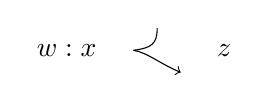
\begin{tikzpicture}[baseline=(x.base)]
\node (x) at (0,0) {$w:x$};
\node at (2,0) {$z$};
\draw (1.15,.28) .. controls (1.15,.08) and (1.08,.03) .. (.85,0);
\draw[->] (.85,0) .. controls (1.03,-.03) and (1.2,-.18) .. (1.45,-.28);
\end{tikzpicture}}.
De plus, on a
\[
x\not\prec x\qquad\left(\text{car }\operatorname{Im}(\Sigma_1\overset{(p_1;\uline{b})}{\unsure{-|\longrightarrow}}\Sigma\times\Sigma)\cap\text{diag}=\varnothing\right)
\]
donc la relation $x\prec y$ est la relation
d'inégalité stricte associée à une relation
d'ordre sur $\Sigma$. On récupère $\Sigma^{<}(1)$ comme
le graphe de la relation d'ordre stricte,
$\Sigma^{<}(2)$ comme les drapeaux $x\prec y\prec z$ de
longueur $2$ dans $\Sigma$, et les applications
\mspage{59}

\scanpage{61}
\mspage{26}
\diagram{\begin{tikzcd}
\Sigma^{<}(1)\arrow[r,shift left=2,"p_1=\uline{s}"]\arrow[r,shift right=2,"\uline{b}"'] & \Sigma
\end{tikzcd}\qquad
\begin{tikzcd}
\Sigma^{<}(2)\arrow[r,shift left=4,"p_2"]\arrow[r,"\uline{s'}" description]\arrow[r,shift right=4,"\uline{b'}"'] & \Sigma^{<}(1)
\end{tikzcd}}
comme
\[
(39)\qquad\left\{\begin{aligned}
(x\prec y)&\xrightarrow{p_1=\uline{s}}x\\
(x\prec y)&\xrightarrow{\uline{b}}y\\
(x\prec y\prec z)&\xrightarrow{p_2}(x,y)\\
(x\prec y\prec z)&\xrightarrow{\uline{s'}}(\deleted{y}\inserted{x},z)\\
(x<y<z)&\xrightarrow{\uline{b'}}(\deleted{x}\inserted{y},z)
\end{aligned}\right.
\]
\uline{Scholie} En résumé, la situation est décrite
par les données suivantes

$1^{\circ})$ Un espace top. \deleted{(séparé)} $\Sigma$, munie d'une stratifica-
tion (pré)cylindrique --- soit $\Sigma_1$ l'espace des strates de
codim $1$, de sorte que $\Sigma^{<}(1)\xrightarrow{\uline{b}}\Sigma$ est une imm. bordante
\inserted{propre}
\margin{``stratification cylindrique localt ordonnée''}

$2^{\circ})$ Une relation d'ordre totale relative de $\Sigma_1$ sur $\Sigma$
(définie par la donnée, pour tt $x\in\uline{b}(\Sigma_1)$, d'un
ordre total sur l'ens des strates de codim $1$
qui passent par $x$, cette relation d'ordre total étant
soumis à la condition d'être \inserted{donnée par} une partie \uline{fermée}
\inserted{$\Sigma^{*}(2)$} de $\bigl((\Sigma^{<}(1),b)\times_\Sigma(\Sigma^{<}(1),b)\ldots\bigr)$ --- soit
\diagram{\begin{tikzcd}
\Sigma^{<}(2)\arrow[r,shift left=2,"\uline{s'}"]\arrow[r,shift right=2,"\uline{b'}"'] & \Sigma^{<}(1)\arrow[r,"\uline{b}"] & \Sigma
\end{tikzcd}}

$3^{\circ})$ Une application continue
\[
p_1\text{ ou }\uline{s}:\Sigma^{<}(1)\longrightarrow\Sigma
\]
ayant les propriétés suivantes

a) $(\uline{s},\uline{b}):\Sigma^{<}(1)\longrightarrow\Sigma\times\Sigma$ est injectif, et
son image ne
rencontre pas la
diagonale \inserted{$\forall\ u\in\Sigma^{<}(1),\ \uline{s}(u)\ne\uline{b}(u)$}
\mspage{60}

\scanpage{62}
b) L'application $\Sigma^{<}(2)\xrightarrow{(p_1\circ s',\unsure{p_1b'})}\Sigma\times\Sigma$
se factorise par $\Sigma^{<}(1)\lhook\joinrel\xrightarrow{(p_1,\uline{b})}\Sigma\times\Sigma$
en un morphisme
\[
p_2:\Sigma^{<}(2)\longrightarrow\Sigma^{<}(1)
\]
qui rende le carré
\diagram{\begin{tikzcd}[column sep=small,execute at end picture={
\draw[densely dotted] ([xshift=7pt]s62sourcea.east) arc[start angle=270,end angle=90,radius=3pt];
\draw[densely dotted] ([xshift=7pt]s62sourceb.east) arc[start angle=270,end angle=90,radius=3pt];}]
|[alias=s62sourcea]|\Sigma^{<}(2)\arrow[rr,"\uline{b'}",start anchor=east,shorten <=7pt]\arrow[dr,"p_2"'] && \Sigma^{<}(1)\arrow[dr,"p_1"]&\\
& |[alias=s62sourceb]|\Sigma^{<}(1)\arrow[rr,"\uline{b}"',start anchor=east,shorten <=7pt] && \Sigma
\end{tikzcd}}
\uline{Cartésien}, et $p_1:\Sigma^{<}(1)\longrightarrow\Sigma$ étant transversal
à \deleted{\unsure{l'imm}}ersion-but $\uline{b}:\Sigma^{<}(1)\longrightarrow\Sigma$.
\margin{\uline{NB} (Si $\Sigma$ est séparé, donc $\Sigma\times\Sigma$ séparé
sur $\Sigma$, et $\Sigma^{<}(1)\xrightarrow{b}\Sigma$
propre, il en résulte
que $\Sigma^{<}(1)\longrightarrow\Sigma\times\Sigma$ est
propre donc un plongement
\uline{fermé}.}
\margin{cette condition de transversalité est
peut-être conséquence des autres\ldots}

De façon équivalente, une telle structure
est donnée par un espace topologique \inserted{séparé} $\Sigma$,
muni d'une relation d'ordre $x\preceq y$
\deleted{dont le graphe est}\inserted{satisfaisant les conditions suivantes}

\deleted{a) le graphe \deleted{$\unsure{\Sigma^{<}(1)}$} $\Sigma(1)$ de cette relation est
fermé dans $\Sigma\times\Sigma$, et $\Sigma(1)\xrightarrow{b}\Sigma$ est
une immersion.
\deleted{$\unsure{\Sigma}$}
b) Si $\Sigma^{*}(1)$ est le graphe de la
relation d'ordre \inserted{stricte}, $\Sigma^{*}(1)\xrightarrow{\uline{b}}\Sigma$ est une
immersion \inserted{bordante} propre \deleted{\unsure{(donc la partie de}}
a) Si $x\in\Sigma$, $\Sigma_{<x}$ \inserted{$(=\Sigma^{*}(1)_x)$}, \deleted{\unsure{est}}
est (fini) \uline{tot.} \uline{ordonné}.
}
\mspage{61}

\scanpage{63}
\mspage{27}
\deleted{c) Si $(z_\alpha)_{\alpha\in I}$ est l'ens des éléments de
$\Sigma_{<x}=\uline{b}^{-1}(\{x\})$ (où $\uline{b}:\Sigma^{<}(1)\longrightarrow\Sigma$), les
\unsure{les}}

a) Pour tt $x\in\Sigma$, l'ens $\Sigma_{<x}$ \deleted{(fini) est}\inserted{est tot${}^t$}
\deleted{$\simeq\uline{b}^{-1}(\{x\})$} ordonné

b) Si $\Sigma^{<}(1)$ est le graphe de la relation
$x<y$, et $\uline{s},\uline{b}:\Sigma^{<}(1)\rightrightarrows\Sigma$ sont les applications
source et but, \deleted{\unsure{---}} l'application $\uline{b}$ est une immer-
sion \deleted{bordante} \uline{propre} (donc les $\Sigma_{<x}=\uline{b}^{-1}(\{x\})$
sont finis)

c) Si $(z_\alpha)_{\alpha\in I}$ sont les éléments de $\Sigma_{<x}=b^{-1}(\{x\})$,
alors \deleted{les}\inserted{la famille} germes \inserted{en $x$} de sous-espaces \deleted{bordants}\inserted{de $\Sigma$}
images par $\uline{b}$ des \inserted{germes} $(\Sigma^{<}(1),z_\alpha)$, \deleted{sont}\inserted{une famille}
\deleted{transversaux}\inserted{transversale}
de sous-espaces \uline{bordants}.

d) $\uline{\unsure{s|b}}:\Sigma^{<}(1)\longrightarrow\Sigma^{\unsure{*}}$ est \uline{transversal} p.v. à l'immersion
bordante $\uline{b}:\Sigma^{<}(1)\longrightarrow\Sigma^{\unsure{*}}$
\deleted{\unsure{la diag}}
\margin{ou sous forme d'une \unsure{récollection|récollement}
pour les $z_\alpha\in\Sigma^{<}(1)$ au dessus d'un même
$x\in\Sigma^*$\ldots}

$1^{\circ})$ Cas équisingulier : $\uline{s}:\Sigma^{<}(1)\longrightarrow\Sigma$ fibrant \inserted{(propre)}

$2^{\circ})$ Cas non singulier : $\Sigma$ est une variété à bord,
dont le bord est $\uline{b}(\Sigma^{*}(1))$.

$3^{\circ})$ Cas équisingulier-non singulier : $\uline{s}:\Sigma^{<}(1)\longrightarrow\Sigma$ est
fibrant, \inserted{propre} à fibres des variétés à bord, et le
fibré des bords est l'image de $\Sigma^{*}(2)$ par
le morphisme $\Sigma^{*}(2)\xrightarrow{\uline{s'}}\Sigma^{*}(1)$ \deleted{\unsure{avec}}\inserted{donné}
par $(x\prec y\prec z)\longrightarrow(x\prec z)$.
\margin{c'est sans doute conséquence de la conjonction des deux conditions $1^{\circ}),2^{\circ})$}
\mspage{62}

\scanpage{64}
Les morphismes les plus importants de la
situation apparaissent dans le diagramme
\inserted{hexagonal} suivant
\diagram{\begin{tikzcd}[column sep=small,row sep=large,execute at end picture={
\draw[densely dotted] ([xshift=7pt]s64upper.east) arc[start angle=270,end angle=90,radius=3pt];
\draw[densely dotted] ([xshift=7pt]s64centre.east) arc[start angle=270,end angle=90,radius=3pt];
\draw[densely dotted] ([xshift=-5pt,yshift=5pt]s64right.north west) arc[start angle=135,end angle=315,radius=3pt];
\draw[densely dotted] ([xshift=7pt]s64lower.east) arc[start angle=270,end angle=90,radius=3pt];}]
&|[alias=s64upper]|\Sigma^{<}(1)\arrow[rr,"\uline{b}",start anchor=east,shorten <=7pt]\arrow[dl,"\uline{s}"']&&\Sigma&\\
\Sigma&&|[alias=s64centre]|\Sigma^{<}(2)\arrow[ul,hook,"\uline{s'}"]\arrow[rr,"\uline{b'}",start anchor=east,shorten <=7pt]\arrow[dl,"p"']\arrow[ur,phantom,"\text{cart}" description]\arrow[dr,phantom,"\text{cart}" description]&&|[alias=s64right]|\Sigma^{<}(1)\arrow[ul,"\uline{b}"',start anchor=north west,shorten <=7pt]\arrow[dl,"\uline{s}"]\\
&|[alias=s64lower]|\Sigma^{<}(1)\arrow[ul,"\uline{s}"]\arrow[rr,"\uline{b}"',start anchor=east,shorten <=7pt]&&\Sigma&
\end{tikzcd}},
(40)

où les flèches marquées \diagram{\begin{tikzcd}[column sep=large,execute at end picture={
\draw[densely dotted] ([xshift=7pt]s64legend.east) arc[start angle=270,end angle=90,radius=3pt];}]
|[alias=s64legend]|{}\arrow[r,start anchor=east,shorten <=7pt]&{}
\end{tikzcd}} (en fait,
$\uline{b},\deleted{\unsure{p_2}},\uline{b'},\uline{s'}$) sont des immersions bordantes, \inserted{propres}
et les flèches marquées $\longrightarrow$ (en fait,
$\uline{s}$ et $p$) sont (dans le cas équisingulier)
fibrantes et propres \unsure{\}} (voire, de plus : fibres
des variétés à bord, dont le bord est
dans le cas de $\uline{s}:\Sigma^{<}(1)\longrightarrow\Sigma$, l'image
de $\Sigma^{<}(2)\overset{\uline{s'}}{-}\Sigma^{<}(1)$\inserted{(i.e. l'ens des $(x\prec y)$ tels que $y$ \uline{ne soit pas} successeur de $x$)}).
\margin{donc, dans le cas de $p:\Sigma^{<}(2)\longrightarrow\Sigma^{<}(1)$,
le fibré des bords est l'image de $\Sigma^{<}(3)$}
On fera attention
que les applications fibrantes $s,p$ n'ont \deleted{\unsure{rien}}\inserted{rien}
de surjectif --- l'image de $s$ est formé des $x\in\Sigma$
qui \uline{ne sont pas maximaux}, celle de $p$ est formé
des $(x\prec y)$ tels que $y$ ne soit pas maximal.
\mspage{63}

\scanpage{65}
\mspage{28}
\uline{12} Récapitulation (des données de déploiement,
relatif à un ens ordonné $I$, fini disons\ldots)

\[
\left\{\begin{aligned}
\text{a) }&\text{Espaces }\Sigma_i\quad(i\in I)\\
\text{b) }&\text{Espaces }\Sigma_{i,j}\quad(i<j,\ i,j\in I)\\
\text{c) }&\text{Applications }\Sigma_{i,j}\xrightarrow{s_{ij}}\Sigma_i,\quad\Sigma_{ij}\xrightarrow{b_{ij}}\Sigma_j
\end{aligned}\right.
\]
\margin{C'est la structure envisagée dans le Scholie (p. $26/27$)
plus une application continue strictement croissante
$\Sigma\xrightarrow{\varphi}I$, telle que $\forall x\in\Sigma$, $\varphi|\Sigma_{<x}$
soit injective (\uline{donc} la relation d'ordre de \inserted{\unsure{(pour $i$ ?)}}
$\Sigma_{<x}$ est induite par celle de $I_{<i}$).}

Conditions

a) $\Sigma_{ij}\longrightarrow\Sigma_j$ \deleted{immersion}\inserted{plongement} fermé \deleted{bordant}
\inserted{[On identifie $\Sigma_{ij}$ à un sous-espace fermé de $\Sigma_j$ par $b_{ij}$]}

b) $\Sigma_{i,k}\cap\Sigma_{j,k}=\varnothing$ si $i,j$, \deleted{$\unsure{\exists}$} non comparables
\deleted{\unsure{(on suppose}}\deleted{\unsure{$i<j$}} (NB $i,j<k$)
\margin{\uline{NB} La condition b) équivaut à celle
que dans l'ens ordonné $\Sigma=\coprod\Sigma_i$, les ensembles
$\Sigma_{<x}$ sont tot${}^t$ ordonnés.}

c) Pour $i<j<k$ posons
\[
\uline{\Sigma_{ijk}=\Sigma_{ik}\cap\Sigma_{jk}\subset\Sigma_k}.
\]
On a alors \inserted{dans $\Sigma_{jk}$ :}\deleted{$\unsure{\Sigma_{jk}}$}
\[
\uline{\Sigma_{ijk}\deleted{\unsure{\ne}}\subset\deleted{\unsure{\Sigma_{ik}}}\unsure{b_{ij}^{-1}|s_{jk}^{-1}}(\Sigma_{ij})}\deleted{\unsure{défini}}
\]
\deleted{\unsure{une}}
On a donc, pour $i<j<k$, un diagramme
commutatif hexagonal
\diagram{\begin{tikzcd}[column sep=small,row sep=large]
&\Sigma_{ik}\arrow[rr,hook,"b_{ik}"]\arrow[dl,"s_{ik}"']&&\Sigma_k&\\
\Sigma_i&&\Sigma_{ijk}\arrow[ul,hook]\arrow[rr,hook]\arrow[dl]\arrow[ur,phantom,"\text{cart}" description]\arrow[dr,phantom,"\text{cart}" description]&&\Sigma_{jk}\arrow[ul,hook,"b_{jk}"']\arrow[dl,"s_{jk}"]\\
&\unsure{\Sigma_{ij}}\arrow[ul,"s_{ij}"]\arrow[rr,hook,"b_{ij}"']&&\Sigma_j&
\end{tikzcd}}
(41)

où les flèches $\hookrightarrow$ sont des inclusions
fermées \inserted{cf plus bas} (bordantes), et les flèches $\longrightarrow$
sont des applications qui seront fibrantes et propres
dans le cas équisingulier.
\mspage{64}

\scanpage{66}
d) \deleted{\unsure{a}} Les $\Sigma_j\hookrightarrow\Sigma_{ji}$ sont bordants, et si
$x\in\Sigma_i$, \deleted{les} donc les $\Sigma_{ji}\ni x$ (\deleted{pour $j<i$}\inserted{indices}
\deleted{tels que}\deleted{$\unsure{\Sigma}$}\inserted{par l'ens} $I_{<i,x}\overset{\mathrm{def}}{=}\{j\in I\mid j<i,\ \Sigma_{ji}\ni x\}$,
qui est totalement ordonné par b)) sont
des sous-espaces-bords transversaux en $x$
--- i.e. les $\Sigma_{ji}$ $(j\in I_{<i})$ sont des
sous-espaces bords de $\Sigma_i$ mutuellement
transversaux.

e) $\Sigma_{ij}\xrightarrow{s_{ij}}\Sigma_i$ est transversal p.v. au système trans-
versal des morphismes bordants
$\unsure{b_{ki}|b_{ik}}:\unsure{\Sigma_{ki}}\longrightarrow\Sigma_i$

Si on pose
\[
\Sigma=\coprod_{i\in I}\Sigma_i
\]
\[
\Sigma^{<}(1)=\coprod_{\substack{i,j\in I\\i<j}}\Sigma_{ij}
\]
et $\uline{s},\uline{b}:\Sigma^{<}(1)\longrightarrow\Sigma$ induits par les
$s_{ij},b_{ij}$, alors les conditions a) b) c)
signifient que $(\uline{s},\uline{b}):\Sigma^{<}(1)\longrightarrow\Sigma\times\Sigma$ est
inj. et a comme \deleted{graphe}\inserted{image} le graphe d'une
relation d'ordre stricte, avec $\uline{b}:\Sigma^{<}(1)\longrightarrow\Sigma$
\inserted{immersion} propre, \deleted{et} que l'application \inserted{continue évidente} $\varphi:\unsure{\Sigma|\Sigma^{*}}\longrightarrow I$
est strict${}^t$ croissante, et que pour tt $x\in\Sigma$,
l'application induite $\varphi:\Sigma_{<x}\longrightarrow I_{<i}$ $(i=\varphi(x))$ est
injective, enfin que $\Sigma_{<x}$ est tot${}^t$ ordonné.
\mspage{65}

\scanpage{67}
\mspage{29}
Enfin, la condition d) signifie que cette structure
\inserted{d'espace top. ordonné}
satisfait la condition c) du Scholie (p. $27$).

\uline{Cas équisingulier} : les $s_{ij}$ sont fibrants propres

\uline{Cas non singulier} : les $\Sigma_i$ sont des variétés
topologiques; le bord de $\Sigma_i$ est la réunion
des $\Sigma_{ji}$ pour $j<i$ \deleted{(NB il suffit
de prendre pour $j$}
\margin{On voudra que les $\Sigma_{ij}$ soient des variétés à bord, que le
bord soit la réunion des $\Sigma_{kij}$ et $\Sigma_{ijk}$ --- mais
c'est sans doute une conséquence de la condition précédente\ldots}

\uline{Cas équisingulier-non singulier}
$\unsure{s_{ij}|s_{jk}}:\unsure{\Sigma_{jk}|\Sigma_{ik}}\longrightarrow\Sigma_j$ est
une fibration propre, à fibres des variétés
à bord, le fibré des bords est réunion
des $\Sigma_{ijk}$ pour $i<j<k$.

13. \uline{Une digression} Revenons au cas de
$\Sigma,\unsure{\Sigma^{*}(1)|\Sigma^{<}(1)}\subset\Sigma\times\Sigma$, sans donnée de $I$. Plus
généralement, considérons une \uline{catégorie topologique}
\[
\uline{\Sigma}=(\Sigma_{(0)}=\operatorname{Ob}(\uline{\Sigma}),\quad\Sigma_{(1)}=\operatorname{Fl}(\uline{\Sigma}),
\]
\diagram{\begin{tikzcd}
\Sigma_{(1)}\arrow[r,shift left=2,"\uline{s}"]\arrow[r,shift right=2,"\uline{b}"']&\Sigma_{(0)}
\end{tikzcd}}
\diagram{\begin{tikzcd}[column sep=large]
(\Sigma_{(1)},b)\times_{\Sigma_{(0)}}(\Sigma_{(1)},s)\arrow[r,Rightarrow,"\text{déf}"] & \Sigma_{(2)}\arrow[r,"\unsure{\text{cpl.}|\text{appl.}}","\text{comp. des flèches}"'] & \Sigma_{(1)}
\end{tikzcd}}
), et supposons
que $\uline{s}:\Sigma_{(1)}\longrightarrow\Sigma_{(0)}$ soit \uline{fibrant}. Je dis
qu'alors $\pi_0(\Sigma_{(0)})=\unsure{I_{(0)}|I}$ est \uline{un ens. \inserted{pré}ordonné},
en prenant comme graphe de la relation
d'ordre l'image de
\diagram{\begin{tikzcd}[column sep=large]
\pi_0(\Sigma_{(1)})\arrow[r,"{\pi_0(\uline{s},\uline{b})}"]&\pi_0(\Sigma_{(0)}\times\Sigma_{(0)})\arrow[d,"\sim"]\\
&\pi_0(\Sigma_{(0)}\times\Sigma_{(0)})
\end{tikzcd}}
\mspage{66}

\scanpage{68}
\deleted{Ceci posé} Cette relation est évidemment \deleted{symétrique}\inserted{réflexive}, et
elle est transitive grâce au fait que
\[
\pi_0(\Sigma_{(2)})\longrightarrow
(\pi_0(\Sigma_{(1)}),\pi_0(\uline{b}))\times_{\pi_0(\Sigma_{(0)})}
(\pi_0(\Sigma_{(1)}),\pi_0(\uline{s}))
\]
est surjective, ce qui est facile à prouver,
grâce à l'hypothèse que $\uline{b}$ est fibrant, par le
\uline{Lemme} : Soit
\diagram{\begin{tikzcd}
X\arrow[d,"f"'] & X'\arrow[l,"f'"']\arrow[d,"g'"]\\
Y & Y'\arrow[l,"g"]
\end{tikzcd}}
un carré
cartésien d'espaces top., avec $f$ fibrant,
alors $\pi_0(X')\longrightarrow\pi_0(X)\times_{\pi_0(Y)}\pi_0(Y')$ est surjectif.
Ceci posé, considérons la catégorie top. discrète associée
à l'ens \inserted{pré}ordonné $I_0$\inserted{$=\pi_0(\Sigma_0)$} que par abus de langage
\inserted{[\unsure{anglicisme}]}
on désignera par $I$. On a alors un foncteur
\inserted{canonique} de catégories topologiques \deleted{canonique}
\[
\uline{\Sigma}\xrightarrow{\uline{\varphi}}I
\]
qui est donc donné par des applications continues
\[
\left\{\begin{aligned}
\Sigma_{(0)}&\xrightarrow{\varphi_0}I_0=I\\
\Sigma_{(1)}&\xrightarrow{\varphi_1}I_1=\text{graphe de la relation d'ordre}
\end{aligned}\right.
\]
\inserted{$=\text{image de }\pi_0(\Sigma_1)$ \deleted{dans $\unsure{\pi_0(\Sigma_1)\times I}$}
dans $\pi_0(\Sigma_0)\times\pi_0(\Sigma_0)=I$}
i.e. des décompositions en sommes directes
\[
\Sigma_{(0)}=\coprod_{i\in I}\Sigma_i
\]
\[
\Sigma_{(1)}=\deleted{\sum}\coprod_{\substack{i,j\in I\\i\leq j}}\Sigma_{ij}
\]
\margin{\uline{NB} on suppose les comp. connexes des $\Sigma_0$ et $\Sigma_1$ ouvertes}
compatibles avec $\uline{s},\uline{b}$
i.e. $\uline{s}:\Sigma_{ij}\longrightarrow\Sigma_i$
$\uline{b}:\Sigma_{ij}\longrightarrow\Sigma_j$
avec $\Sigma_{(0)}\xrightarrow{\delta}\Sigma_{(1)}$ ($\delta(x)=\deleted{\unsure{\Sigma}}\operatorname{id}^{\uline{\Sigma}}_x$)
appliquant $\Sigma_i$ dans $\Sigma_{ii}$, \deleted{\unsure{et ainsi}} ce qui
implique déjà la compatibilité de $\varphi=(\varphi_0,\varphi_1)$ avec
la composition). De plus, $\varphi$ est un
\mspage{67}

\scanpage{69}
\mspage{30}
\uline{propriété universelle} évidente pour les morphismes
de la catégorie topologique $\uline{\Sigma}$ dans un ens. \inserted{pré}ordonné.
\unsure{\S} Supposons maintenant que $\uline{\Sigma}$ satisfasse les
conditions
\inserted{\unsure{c}}
\deleted{a) toute flèche inversible de $\uline{\Sigma}$ est
une identité}
\deleted{a) L'application $\delta:\Sigma_0\longrightarrow\Sigma_1$ est
un plongement ouvert et fermé. C'est le cas
si p.ex. $\uline{b}:\Sigma_1\longrightarrow\Sigma_0$ est une immersion
propre\ldots.}

a) $\Sigma_{(1)}\xrightarrow{\uline{b}}\Sigma_{(0)}$ est une immersion
propre ($\Longrightarrow\ \delta:\Sigma_{(0)}\longrightarrow\Sigma_{(1)}$ est une imm.
ouverte et fermée, en sorte que \deleted{$\Sigma_{(1)}=\delta(\Sigma_{(0)})\amalg$}
\[
\Sigma_{(1)}\simeq\delta(\Sigma_{(0)})\amalg\Sigma^{*}(1)
\]
)

b) $\Sigma^{*}_{(1)}\xrightarrow{\uline{b}|\Sigma^{*}(1)}\Sigma_{(0)}$ est une immersion à image
localt \uline{rare} i.e. à intérieur vide\ldots

c) \deleted{\unsure{---}} Toute composante connexe de $\Sigma_{(0)}$ est de
dim finie.
Alors on trouve que $\Sigma_{ii}^{*}\overset{\mathrm{déf}}{=}\Sigma_{ii}\cap\Sigma^{*}(1)=\varnothing$,
par des raisons de dimension (car $\Sigma_{ii}^{*}$ est
fibré sur \deleted{sur} $\Sigma_i$, donc s'il est non vide, de
dim $\geq\dim\Sigma_i$; mais comme $\Sigma_{ii}^{*}\longrightarrow\Sigma_i^{*}$ est
une imm. v.v., on doit avoir aussi $\dim\Sigma_{ii}^{*}<$
$\dim\Sigma_i^{*}$, donc $\unsure{\Sigma_{ii}^{<}|\Sigma_{ii}^{*}}$ est vide), i.e.
\[
\boxed{\Sigma_i\xrightarrow{\sim}\Sigma_{ii}}:
\]
toute flèche \deleted{dans} entre deux
\deleted{\unsure{objets de}} éléments de $\Sigma_{(0)}$ qui sont dans une
même composante connexe \deleted{sont} est une identité.
\mspage{68}

\scanpage{70}
Supposons \unsure{en|de} plus

d) toute flèche inversible de $\uline{\Sigma}$ est une identité
(p.ex. $\uline{\Sigma}$ est une catégorie définie par un ens
\uline{ordonné}).

Alors on conclut aisément que l'ens. pré-ordonné $I$ est
\uline{ordonné}, et que tte flèche de $\uline{\Sigma}$ qui n'est pas
une identité i.e. $u\in\Sigma^{*}(1)$, son image dans $I(1)$
n'est pas une identité;
\deleted{\unsure{i.e.}} Si $\uline{\Sigma}$ est associé à un
\deleted{\unsure{ens. ord.}}\inserted{espace top.}
ordonné, $\Sigma=\Sigma_{(0)}$, cela signifie que
$\uline{\Sigma}\longrightarrow\uline{I}$ est \inserted{une appl.}
\uline{strictement} croissante.

Revenons alors à un \deleted{catég} ens. ordonné topologique
\[
\uline{\Sigma}=(\Sigma=\Sigma_{(0)},\quad
\underset{\underset{\Sigma\times\Sigma}{\cap}}{\Sigma_{(1)}}
=\delta(\Sigma_{(0)})\amalg\Sigma^{<}(1))
\]
satisfaisant aux conditions a) b) c) et 1°) de la page (27)
(correspondant \inserted{localement} à un déploiement d'une
stratification locale équisingulier), et tel que les comp. connexes
de $\Sigma$ \deleted{sont} de dim finie.
Considérons alors le \deleted{foncteur}\inserted{morphisme}
canonique $\uline{\Sigma}\longrightarrow\uline{I}$ avec $I=\pi_0(\Sigma)$,
et supposons de plus que pour $i<j$ ($i,j\in I$)
\[
\Sigma_{ij}\longrightarrow\Sigma_j\quad\hbox{soit \uline{mono} i.e. plongement fermé.}
\]
On est alors sous les conditions de p. 28,
données a) b) c)
$(\Sigma_i,\Sigma_{ij},\ s_{ij},b_{ij}:$
\diagram{\begin{tikzcd}[column sep=large,row sep=small]
&\Sigma_i\\
\Sigma_{ij}\arrow[ur]\arrow[dr]&\\
&\Sigma_j
\end{tikzcd}}$)$,
\mspage{69}

\scanpage{71}
\mspage{31}
satisfaisant les conditions a) c), \inserted{d)} de p. 28.
A-t-on aussi la condition b) de p. 28
\[
\Sigma_{ik}\cap\Sigma_{jk}=\varnothing\quad\hbox{si }i,j<k,\quad
i,j\ \hbox{non comparables ?}
\]
Si on avait $x\in\Sigma_{ik}\cap\Sigma_{jk}\subset\Sigma_k$,
alors on aurait deux éléments $\unsure{x_i}$ et $y$ de $\Sigma$,
au dessus de $i$ et $j$ respectivement, qui sont $<x$
(au dessus de $k$), donc (comme $\Sigma_{<x}$ est tot\textsuperscript{t} ordonné)
\deleted{on aurait} $x$ et $y$ seraient comparables, donc aussi
$i$ et $j$, absurde.

\uline{Conséquence} les structures ``déploiements
équisinguliers de stratifications, indexés par $I$'',
décrites \deleted{dans} la p. 28, équivalent à la structure suivante :

\margin{\unsure{et|si} les comp. connexes des $\Sigma_i$ sont de dim finie.}

\textcircled{a} Un \deleted{$\Sigma$} espace top. ordonné $\Sigma$,
satisfaisant aux conditions a) b) c) et 1°) de la page 27,
et \uline{de plus} : la condition que, \deleted{pour tout}
posant $\widetilde I=\pi_0(\Sigma)$, on ait, pour
$i,j\in\widetilde I$, $i<j$, que le morphisme d'immersion
propre bordant $\Sigma_{ij}\xrightarrow{b_{ij}}\Sigma_j$ soit
\uline{mono}

\textcircled{b} Une application strictement croissante
(\unsure{pas néc.} surjection)
\[
\widetilde I\longrightarrow I
\]
\mspage{70}

\scanpage{72}
\uline{Remarque} Dans deux contextes différents
``déploiement''$^{*}$ de \deleted{\unsure{strag}} stratifications, on
a rencontré des espaces topologiques ordonnés\inserted{$\Sigma$},
satisfaisant les conditions suivantes

\margin{$*$ en deux sens assez différents}

a) $\Sigma_{(1)}\xrightarrow{\uline{s}}\Sigma_{\unsure{*|0}}=\Sigma_{(0)}$
est une fibration propre

b) $\Sigma_{(1)}\xrightarrow{\uline{b}}\Sigma_{(0)}$ est une immersion propre

c) Si $x,y\in\Sigma$ sont ds une $\unsure{\overline{\mathrm m}}$ composante connexe,
alors $x\leq y\Longrightarrow x=y$
\inserted{(i.e. si $x,y\in\Sigma$, $x<y$, alors $x,y$ sont dans deux
composantes connexes différentes)}

\margin{conséquence de a) b) si on suppose que
$\Sigma(1)^{*}\xrightarrow{\uline b}\Sigma$ est \uline{\unsure{rare}},
et que les comp. connexes de $\Sigma$ de dim finie\ldots}

Dans un cas (celui d'une notion assez \unsure{anodine|analogue à}
\unsure{de la notion|la notion} de déploiement d'une stratification de type $I$ disons,
par $\Sigma=\coprod X_i$,
$\Sigma_1=\displaystyle\coprod_{\substack{i,j\text{ tels que}\\X_i\subset X_j}}X_i$),
$\uline s$ est étale, (\unsure{localt} fini donc) et rien de plus spécial pour $\uline b$.
Dans le cas de la théorie \deleted{\unsure{proposée}}\inserted{développée}
ici des déploiements\inserted{de stratifications équisingulières},
$\uline b$ est bordant, rien de spécial sur $\uline s$.
Dans l'un et l'autre cas, on peut appliquer la sorite
sur $\widetilde I=\pi_0(\Sigma)$ --- dans le premier cas,
cela revient à \unsure{remplacer|raffiner} la stratification par les $X_i$ par celle
par les comp. connexes des $X_i$ (donnant un $\widetilde I$;
dans le deuxième,
\deleted{à \unsure{remplacer|raffiner} \unsure{ito} $\unsure{\Longleftarrow}$ \unsure{exact}}
itou pour les
\[
X_i^{*}=X_i\setminus\bigcup_{j<i}\unsure{X_{ij}|X_j}.
\]
\mspage{71}

\scanpage{73}
\mspage{32}
14. \uline{Description heuristique des} $\Sigma_i,\Sigma_{ij}$.
(Peut se préciser considérablement \unsure{ds|dans} un contexte de topologie modérée).
Pour construire $\Sigma_i$, on prend un voisinage tubulaire
\inserted{``standart'' $T_{<i}$} fermé de
$\unsure{\dot X_i|\dot\Sigma_i}=\displaystyle\bigcup_{k<i}X_i$, et on prend
\[
(42)\qquad\Sigma_i=X_i\setminus X_i\cap\mathring T_{<i}.
\]
\[
\mathring T_{<i}\overset{\mathrm{déf}}{=}T_{<i}\setminus\dot T_{<i}.
\]
\margin{\uline{NB} On peut prendre $T_{<i}=\bigcup_{k<i}T_k$,
où $T_k$ est un vois. tub. standart des $X_k$}
(\uline{NB} Il aurait suffit ici de prendre le voisinage tubulaire
standart dans $X_i$ lui-m\textsuperscript{e}, et de prendre donc
$\Sigma_i=X_i\setminus\mathring T_{<i}$)

Pour construire $\Sigma_{ij}$, on prend un voisinage tubulaire
$T'_{ij}$ de $\Sigma_i$ dans
$X_j\setminus X_j\cap\unsure{\mathring T_{<i}|\mathring T_{<i0}}=X'_i$
(NB cette fois-ci il faut \deleted{prendre} d'abord prendre
$T_{<i}$ vois. tub. standart \uline{ds} $X$, ou sinon, ds $X_j$).
On prend $T'_{ij}$ ``suffisamment petit'' p.r. au choix de $T_{<i}$.
Puis on prend $\dot T'_{ij}$\deleted{\unsure{s}}, et dans $\dot T'_{ij}$
la trace de $\displaystyle\bigcup_{\unsure{i<k<j|i\leq k<j}}X_{jk}$
(cela est vide si $j$ est un successeur de $i$), soit $S\dot T'_{ij}$
(``partie singulière'' de $T'_{ij}$.

\figure{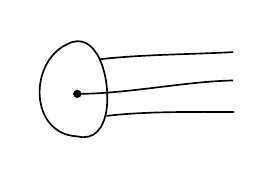
\begin{tikzpicture}[x=1cm,y=1cm,line width=.6pt]
\draw (0.05,-.58) .. controls (-.56,-.55) and (-.57,.36) .. (-.08,.59)
.. controls (.29,.79) and (.48,.18) .. (.42,-.25)
.. controls (.38,-.49) and (.26,-.63) .. (.05,-.58);
\draw (.34,.40) .. controls (.87,.46) and (1.45,.46) .. (2.03,.49);
\draw (.06,-.04) .. controls (.68,-.04) and (1.44,.12) .. (2.03,.13);
\draw (.42,-.32) .. controls (.92,-.26) and (1.55,-.27) .. (2.04,-.27);
\fill (.05,-.04) circle (1.5pt);
\end{tikzpicture}}

On prend alors un voisinage tubulaire standart
\inserted{$T(S\dot T'_{ij})$} de $S\dot T'_{ij}$ dans $\dot T'_{ij}$,
qu'on peut supposer induit par la réunion \inserted{$\bigcup T_k$}
des voisinages tubulaires standart des $X_k$ ($i<k<j$)
dans $\unsure{X---X_j}$
(pris ``assez petits'' p.r. aux choix déjà faits de $T_{<i}$
et \inserted{de} $T'_{ij}$).
On \deleted{prend}\inserted{aura} alors
\[
(43)\qquad\Sigma_{ij}=\dot T'_{ij}\setminus\mathring T(S\dot T'_{ij})
\]
\mspage{72}

\scanpage{74}
de sorte qu'on aura
\[
\Sigma_{ij}\subset\Sigma_j
\]
\margin{à condition d'avoir ajusté de façon cohérente les choix
qui donnent $\Sigma_i,\Sigma_{ij}$.}
\deleted{Cette construction \unsure{devra}}

Pour ajuster les choix, de façon à avoir,
\deleted{\unsure{des}}\inserted{disons}
$i<j<k$, des $\Sigma_{ik}$ et $\Sigma_{jk}$ dans $\Sigma_k$ en
\deleted{relations de la forme}
position relative correcte, de sorte que leur intersection
mérite le nom de $\Sigma_{ijk}$,
On introduit comme plus haut une ``fonction dimension'' sur $I$;
\deleted{qui soit}
\deleted{$I_0=$ \unsure{ens}}
\[
I\xrightarrow{\delta}\mathbb N
\]
qui soit \uline{strictement croissante}, \deleted{et on}
(on ne lui en demande pas plus),
\deleted{et on construit}
\deleted{(posant $X_{(d)}=\bigcup_{\delta(i)\leq d}X_i$)}
\deleted{$T_0$ voisinage tubulaire standart de
$X_{(0)}=\bigcup_{\substack{i\in I\\\delta(i)=0}}X_i$

$T_1$ voisinage tubulaire standart de
$X_{(1)}\setminus\mathring T_0\unsure{=}$
\deleted{$\unsure{X\setminus\mathring T_0}$}\inserted{$\unsure{X^{(0)}_{(0)}}$}
dans $X^{(1)}=X\setminus\dot X_{(0)}$}

On pose, pour $d\in\mathbb Z$
\[
(44)\qquad X_{(d)}=\bigcup_{\substack{i\in I\\\delta(i)\leq d}}X_i
\]
\deleted{On}
\[
(45)\qquad X_{-1}=\varnothing\subset X_{(0)}\subset X_{(1)}\ldots
\subset X_{(N)}=X\quad\hbox{si }N=\operatorname{Sup}_{i\in I}\delta(i)
\]
On construit par récurrence une filtration décroissante par des
\uline{fermés}
\[
(46)\qquad X^{(0)}=X\supset X^{(1)}\supset\ldots\supset X^{(N+1)}=\varnothing
\]
avec
\[
(47)\qquad X^{(i)}\subset X\setminus X_{i-1}
\]
i.e.
\[
X^{(1)}\subset X\setminus X_{(0)},\quad
X^{(2)}\subset X\setminus X_{(1)},\quad\ldots\quad
X^{(N+1)}\subset X\setminus X_{(N)}=X-X=\varnothing
\]
\mspage{73}

\scanpage{75}
\mspage{33}
On choisit un voisinage tubulaire standart $T_{(0)}$ de
$X_{(0)}$ dans $X$, et on pose
\[
\deleted{(\unsure{48})}\qquad
\left\{\begin{aligned}
X^{(1)}_{\deleted{\unsure{i}}}&=X\setminus\mathring T_{(0)}\\
X^{(1)}_{(d)}&=X^{(1)}\cap X_{(d)}\qquad(=\varnothing\text{ si }d\leq0)\\
X^{(1)}_i&=X^{(1)}\cap X_i
\end{aligned}\right.
\]
\margin{de sorte que $X^{(1)}_{(d)}=\displaystyle\bigcup_{\substack{i\in I\\\delta(i)\leq d}}X^{(1)}\cap X_i$}

On \deleted{pose}\inserted{prend} alors un voisinage tubulaire
standart \deleted{de} $T_1^{\deleted{\unsure{1}}}$ de $X_{(1)}$ dans $X$
(petit par rapport au choix de $T_0$), soit $T_1^{(1)}$ sa trace dans
$X^{(1)}$, qui est un vois. tub. standart de $X^{(1)}_{(1)}$ dans
$\unsure{x^{(1)}|X^{(1)}}$. On pose
\[
\deleted{(\unsure{49})}\qquad
\begin{aligned}
X^{(2)}&=X^{(1)}\setminus\mathring T^{(1)}_{(1)}
=X^{(1)}\cap(X\setminus\mathring T_1)\\
&=X^{\deleted{\unsure{2}}}\setminus(\mathring T_0\cup\mathring T_1)
\end{aligned}
\]
\margin{NB $T_d=\displaystyle\bigcup_{\substack{i\in I\\\delta(i)\leq d}}T_i$,
où $T_i$ est un vois. tub. de $X_i$ dans $X$}

On prend un voisinage tubulaire $T_d$ de $X_{(d)}$ dans $X$,
petit p.r. aux vois. tubulaires $T_{d'}$ ($d'<d$) déjà construits,
et on pose
\[
(48)\qquad X^{(d)}=X-\bigcup_{\alpha<d}\mathring T_\alpha.
\]
Ceci posé, on pose, pour $i\in I$, $d=\delta(i)$
\[
(49)\qquad\unsure{|}\quad
\begin{aligned}
\Sigma_i&=X_i\cap X_{(d)}
=X_i\setminus\deleted{\unsure{\{}}\bigcup_{\uline{\alpha}<d}X_i\cap
\unsure{\dot T_\alpha|\mathring T_\alpha}
\qquad\deleted{\subset X_i}\\
&=X_i\setminus\bigcup_{\underset{\sim}{j}<i}X_i\cap\mathring T_j
\qquad\subset X_i^*
\end{aligned}
\]
\mspage{74}

\scanpage{76}
Si $i<j$, \deleted{$d=\delta(i),\ d'=\delta(j)$}
\[
(49)\qquad\Sigma_{ij}=\deleted{\unsure{\dot T_j|\dot T_{ij}}\cap\Sigma_j}
\dot T_i\cap\Sigma_j\quad\subset\Sigma_j
\]
et pour un drapeau $i_0<i_1\ldots<i_n$
\[
(50)\qquad\begin{aligned}
\Sigma_{i_0\ldots i_n}&=\dot T_{i_0}\cap\dot T_{i_1}\cap\ldots\cap
\dot T_{i_{n-1}}\cap\Sigma_{i_n}\\
&=\Sigma_{i_0i_n}\cap\Sigma_{i_1i_n}\ldots\cap\Sigma_{i_{n-1}i_n}
\end{aligned}
\]
On a \inserted{de façon évidente} les morphismes de transition
\inserted{entre les $\Sigma_{i_0\ldots i_n}$} pour les
\deleted{\unsure{morphismes}} inclusions \uline{cofinales} de drapeaux,
mais non pour des inclusions quelconques, dont la définition dépend
du choix de rétractions des
\[
T_i^{(d)}=T_i\cap X^{(d)}\qquad d=\delta(i)
\]
sur $X_i^{(d)}=X_i\cap X^{(d)}$, ce qui donne alors
\deleted{\unsure{t}}
\[
\Sigma_{ij}\subset\dot T_i^{(d)}\subset T_i^{(d)}
\longrightarrow X_i^{(d)}=\Sigma_i
\]
la structure complète
$(\Sigma_i,(\Sigma_j),$
\diagram{\begin{tikzcd}[column sep=large,row sep=small]
&\Sigma_j\\
\Sigma_{ij}\arrow[ur]\arrow[dr]&\\
&\Sigma_i
\end{tikzcd}}$)$
(Mais il faut des hyp. d'équisingularité sur la
\deleted{\unsure{f}} stratification de $X$ par les $X_i$,
et une condition \inserted{de \unsure{locale} trivialité}
sur les rétractions
$T_i^{(d)}\longrightarrow X_i$ i.e. \inserted{sur les}
$T_{(d)}^{(d)}\longrightarrow X_{(d)}^{(d)}$,
pour que les $\Sigma_{ij}\unsure{-|\longrightarrow}\Sigma_i$ soient des fibrations)

....
\mspage{75}

\scanpage{77}
\mspage{34}
\uline{15}. Introduction des proespaces :
$V_{i_0\ldots i_n},\ V_J^{\deleted{\unsure{*}}\unsure{L}}$,

On désigne par $V_i^{\unsure{\deleted{*}|*}}$ le
\inserted{pro}voisinage tubulaire (au sens des proespaces)
de $X_i^*=X_i\setminus\bigcup_{j<i}X_j$ dans $X$.
Ainsi, \deleted{\unsure{on}} on a
\[
(51)\qquad X_i^*\longrightarrow V_i^{\unsure{\deleted{*}|*}}
\qquad\text{équivalence d'homotopie de proespaces.}
\]
\deleted{Pour un drapeau}
Si $\unsure{\forall i,j|(i,j)}$ $i<j$, on pose
\[
(52)\qquad\deleted{X_{ij}}\inserted{V_{ij}}=V_i\cap V_j
\]
\margin{Pourquoi
\diagram{\begin{tikzcd}[column sep=small]
V_{ij}^{\unsure{b}}=V_i\cap X_j^*\arrow[r,hook]&{}
\end{tikzcd}}
\unsure{est une|est-ce une} équivalence d'homotopie ?}

\margin{NB $V_{ij}$ a un sens \deleted{\unsure{si}} si $i\neq j$
mais si $i$ et $j$ ne sont pas comparables, on a $V_i\cap V_j=\varnothing$,
\inserted{(du moins si les ouverts de $X$ sont normaux, p.ex. $X$ métrisable)}
si $i=j$, on a $V_{ii}=V_i$}

de sorte qu'on a
\diagram{\begin{tikzcd}[column sep=large,row sep=large]
&V_{ij}\arrow[r,"b_{ij}"]\arrow[d,leftrightarrow,"s_{ij}"]&V_j\\
(X_i\quad\deleted{\longleftarrow}\arrow[r,"{\substack{(w)\\\sim}}"]&)V_i&
\end{tikzcd}}
On a :
\[
(53)\qquad X=\varinjlim(V_i,V_{ij},\deleted{\unsure{\}}}\ b_{ij},s_{ij})
\]
$X$ est obtenu par \uline{recollement} des $V_i$ suivant les $V_{ij}$.

On définit aussi, plus généralement, les
\[
(54)\qquad V_{i_0\ldots i_n}=V_{i_0}\cap\ldots\cap V_{i_n}
\]
pour un drapeau $i_0<i_1<\ldots<i_n$
\margin{\uline{NB} L'expression a un sens \unsure{même} si
l'ens. $\{i_0,\ldots,i_n\}$ ne forme pas un drapeau,
mais il est vide si \unsure{ce} n'est pas un drapeau}
\mspage{76}

\scanpage{78}
C'est un système inductif de \deleted{\unsure{espaces}} proespaces
sur l'ens ordonné opposé de celui des drapeaux de $I$
(pour l'inclusion), dont le $\uline{\lim}$ est \unsure{égalt} $\approx X$.

Soit $Z$ \deleted{$X$} une partie (\inserted{loc\textsuperscript{t}}fermée)
de $X$, et posons, pour \deleted{$\unsure{\forall}$} un $i$ tel que
$\unsure{X_i^*|V_i}\subset Z$
\[
(55)\qquad V_i^Z=V_i\cap Z\qquad
\text{provoisinage tubulaire de }X_i^*\text{ dans }Z
\]
\deleted{de}
On a
\[
(56)\qquad X_i^*\hookrightarrow V_i^Z\hookrightarrow V_i
\qquad\text{équivalences d'homotopie}
\]
Plus généralement, on pose (si $X_{i_n}\subset Z$)
\[
V_{i_0\ldots i_n}^Z=V_{i_0\ldots i_n}\cap Z
=V_{i_0}^Z\cap\ldots\cap V_{i_n}^Z
\]
C'est aussi le $V_{i_0\ldots i_n}$ relatif à la \deleted{fil}
stratification de $Z$ induite par les
$Z_i\overset{\mathrm{déf}}{=}X_i\cap Z$, pour le système d'indices
$i_0\ldots i_n$. On a
\[
(57)\qquad V_{i_0\ldots i_n}^Z\hookrightarrow V_{i_0\ldots i_n}
\qquad\text{équiv. d'homotopie}
\]
Soit $J$ une partie de $I$, posons
\[
(58)\qquad X_J^*=\bigcup_{i\in J}X_i^*,\qquad X_J=\bigcup_{i\in J}X_i
\]
\mspage{77}

\scanpage{79}
\mspage{35}
Si $J$ est un ``idéal'' i.e. $i\in J$, $j<i\Longrightarrow j\in J$,
alors on a $X_J^*=X_J$, donc $X_J^*$ est fermé.
Si $J$ est une ``bande'' i.e. si $i,j\in J$, $i<j$,
alors $\forall k\in I$, $(i<k<j\Longrightarrow k\in J)$,
ou ce qui revient au $=$, si $J'=\widetilde J\setminus J$ est
un ``idéal'', où $\widetilde J$ est l'idéal engendré par $J$,
alors on a
\[
(59)\qquad X_J^*=X_{\widetilde J}^*\setminus X_{J'}^*
\]
\deleted{$=X_{\unsure{\widetilde J|J}}^*$}.
\margin{différence de deux parties fermées, i.e. une partie
loc\textsuperscript{t} fermée de $X$}
dont les $X_i^J\overset{\mathrm{déf}}{=}X_i\cap X_J^*$ ($i\in J$)
forment une stratification. Posons
\[
(60)\qquad V_{j_0\ldots j_n}^J
=V_{j_0\ldots j_n}\cap X_J^*=V_{j_0\ldots j_n}^Z
\qquad\text{pour }Z=X_J^*
\]
pour $j_0\ldots j_n\in J$, $j_0<j_1<\ldots<j_n$,
\deleted{dans la}
ce sont alors les $V_{i_0\ldots i_n}$ associés à la stratification
de type $J$ de $X_J^*=Z$. On a donc
\[
(61)\qquad\begin{aligned}
X_J^*&\simeq\underset{i,j\in J}{\unsure{\varinjlim|\uline{\lim}}}
(V_i^J,V_{ij}^J)\\
&\simeq\underset{\substack{(i_0<\ldots<i_n)\\\in\operatorname{Drap}(J)}}{\uline{\lim}}
(V_{i_0\ldots i_n}^J)
\end{aligned}
\]
\deleted{On s'intéresse à la situation de}
\mspage{78}

\scanpage{80}

\deleted{
deux bandes $J\subset J'$, d'où
\[
X_J^*\subset X_{J'}^*
\]
et à regarder le \inserted{pro}voisinage \deleted{pro}tubulaire de $X_J^*$ dans $X_{J'}^*$, on trouve

\margin{On pourrait les noter $V_J^{J'}$.}
\diagram{\begin{tikzcd}[column sep=small,row sep=small,execute at end picture={
\draw ([xshift=-5pt]s80oval.west)
.. controls ([xshift=-5pt]s80oval.north west) and ([yshift=4pt]s80oval.north west) .. ([yshift=4pt]s80oval.north)
.. controls ([yshift=4pt]s80oval.north east) and ([xshift=5pt]s80oval.north east) .. ([xshift=5pt]s80oval.east)
.. controls ([xshift=5pt]s80oval.south east) and ([yshift=-4pt]s80oval.south east) .. ([yshift=-4pt]s80oval.south)
.. controls ([yshift=-4pt]s80oval.south west) and ([xshift=-5pt]s80oval.south west) .. cycle;
}]
& V_{X_J^*,X_{J'}^*}^{\deleted{\unsure{*}}}=\displaystyle\varinjlim_{i,j\in J\atop\deleted{\unsure{i,j\in J'}}}(V_i^{J'},V_{ij}^{J'}) \quad (62)\\
|[alias=s80oval]|\left(X_J^*=\displaystyle\varinjlim_{i,j\in J}(V_i^J,V_{ij}^J)\right)\arrow[ur,"{\substack{(w)\\\sim}}",bend left=12] &
\end{tikzcd}}

(\uline{NB} \unsure{OPS} $J'=I$, \inserted{de plus} $J$ un idéal dans $J'=I$, quitte à \unsure{rapetisser} $I$ en enlevant $J_0^*=\widetilde J\setminus J$; \deleted{$\unsure{\}}$} \deleted{\unsure{Rem.}} \inserted{ou encore,} on est ramené au cas où on a
\[
\unsure{J_0|I_0}\subset J_1\subset J_2
\]
trois idéaux de $I$, où
\[
J=J_1\setminus J_0,\quad J'=J_2\setminus J_0\quad\ldots
\]
).

\margin{On a $V_J^{J'}=V_J^{J_0'}$, si $J\subset J_0'\subset J'$ est formé des $j\in J'$ qui \unsure{majorent|minorent} un élément de $J$. La condition $\unsure{J'|J}=J_0'$ \unsure{signifie} que $X_J^*$ est fermé dans $X_{J'}^*$, car $J$ est un idéal de $J'$.}

Soit Maintenant, de plus, $K\subset I$ une partie de $I$, et considérons
\[
\deleted{V_J^{J'}\unsure{\setminus X_K\cap V_J^{J'}|_{K}}=\unsure{V(X_J^*)}}
\]
\inserted{$(V_J^{J'}\setminus X_{\unsure{K|k}}\cap V_J^{J'}=)$}
\[
V_{J;K}^{J'}=V(X_J^*,X_{J'}^*)\setminus X_K\cap V(X_J^*,X_{J'}^*)
\]
Notons que pour $k\in I$
\[
(63)\qquad V_{J\deleted{\unsure{;}} ,k}^{J'}\overset{\mathrm{déf}}{=}V_J^{J'}\cap X_k=\varnothing
\quad\overset{\inserted{\text{$X_k$ fermé}}}{\Longleftrightarrow}\quad X_J^*\cap X_k=\varnothing
\]
\[
\deleted{\Longleftrightarrow\unsure{X_k\subset\widetilde J|X_k=\varnothing}}
\]
\[
\deleted{\Longleftarrow\forall i\in I,\quad i\leq k\Rightarrow i\notin J}
\]
\deleted{et \unsure{ce}} et comme $X_k$ est la réunion (disjointe) des $X_i^*$ pour $i\leq k$, La relation (63) est conséquence de celle que \deleted{\unsure{si}} $i\leq k\Rightarrow i\notin J$ i.e. du \deleted{fait pour $k$}
}
\mspage{79}

\scanpage{81}
\mspage{36}

\deleted{le cas \unsure{de|où} $V$}

Posons, pour une bande $J$
\[
\begin{aligned}
(62)\qquad V_J&=\text{provoisinage tubulaire de }X_J^*\text{ dans }X\\
&=\bigcup_{i\in J}V_i=\unsure{\varinjlim|\uline{\lim}}_{i,j\in J}(V_i,V_{ij})
\end{aligned}
\]
On s'intéresse aux \unsure{protopos} de la forme
\[
(63)\qquad V_J^L\overset{\mathrm{déf}}{=}V_J\cap X_L^*,
\]
\margin{\uline{Ex} $J\subset\deleted{J'}\inserted{K\ \text{(idéal de $J'$)}}$ inclusion de bandes, \deleted{d'où} \deleted{\unsure{considérons|voisinage}} $X_J^*\subset X_{J'}^*$, on prend
$V(X_J^*,X_{J'}^*)\setminus V(X_J^*,X_{J'}^*)\cap X_K^*$.}
\margin{\unsure{protopos} de raccord entre $X_J^*$ et $X_L^*$.
\diagram{\begin{tikzcd}[column sep=small,row sep=small]
V_J^L\arrow[r,hook]\arrow[d,hook]&X_L^*\arrow[r,hook]&V_L\\
V_J&&
\end{tikzcd}}
\deleted{$\unsure{V_J\cap V_L=V_{J\cap L}|V_J\cap V_{J'}=V_{J\cap J'}}$}}
où $J,L$ sont deux bandes. Par exemple on \unsure{retrouve} les $X_J^*$ comme
\[
(64)\qquad V_J^J=X_J^*
\]
Soit $L_0\subset L$ l'ens des $l\in L$ qui majorent un élément de $J$, et $J_0$ l'ens des $j\in J$ qui minorent un élément de $L$, on a donc
\[
(65)\qquad V_J^L=V_J^{L_0}=V_{J_0}^L=V_{J_0}^{L_0}
\]
où $J_0,L_0$ sont des sous-bandes de $J,L$ respectivement ($J_0$ est = un idéal de $J$, $L_0$ un coidéal de $L$) telles que \unsure{tt} élément de $J_0$ est majoré par un élément de $L_0$, \unsure{tt} élément de $L_0$ majore un élément de $J_0$. On est ainsi ramené au cas de bandes dans la relation de domination
\[
(66)\qquad J\prec L
\]
\margin{qui signifie que \unsure{tt} élément de $J$ est majoré par un élément de $L$, \unsure{tt} élément de $L$ majore un él. de $J$.}
de
\mspage{80}

\scanpage{82}
\mspage{37}

\uline{Lemme} Soient $I$ un ens ordonné, $J,L$ deux parties de $I$. Conditions équivalentes

a) $1^{\mathrm o})$ $J,L$ sont des bandes, $2^{\mathrm o})$ tout élément de $J$ est majoré par un élément de $L$, tout élément de $L$ majore un élément de $J$, \deleted{$3^{\mathrm o})$ si $j\in J$, $l\in L$ sont tels que $l<j$, alors $j,l\in J\cap L$ !}
\margin{i.e. $J\prec L$}

b) $\exists$ une bande $I'$ de $I$, telle que $J$ soit un idéal de $I'$, $L$ un coidéal de $I'$, et que tout élément de $I'$ majore un élément de $J$ et soit majoré par un élément de $L$.

Sous ces conditions, \deleted{il existe \unsure{une plus}} \inserted{la bande $I'$ de b) est unique, \unsure{plus petite}} petite bande \inserted{$I'$} contenant $J$ et $L$ satisfait b), et est donnée par
\[
(67)\qquad I'=\{i\in I\mid\exists j\in J,l\in L\text{ avec }j\leq i\leq l\}
\]

\uuline{Dém} L'implication b) $\Rightarrow$ a) triviale, \inserted{ainsi que le fait que $I'$ est donné par (67),} prouvons a) $\Rightarrow$ b). Soit $I'$ donné par (67), on a $I'\supset J\cup L$ (par a) $2^{\mathrm o})$) $I'$ est une bande (trivial), et c'est évidemment la plus petite bande $\supset J\cup L$. Prouvons que $J$ est un idéal de $I'$ i.e. $j\in J$, $i\in I'$, $i\leq j\Rightarrow i\in J$.. Comme $i\in I'$, $\exists j_0\in J$ tel que $j_0\leq i$, donc $j_0\leq i\leq j$ avec $j_0,j\in J$, et comme $J$ est une bande \inserted{(par a $1^{\mathrm o})$)} on a $i\in J$. \unsure{On voit} directement que $L$ est un coidéal de $I'$. Soit $i\in I'$, \deleted{\unsure{de par}} définition de $I'$ $i$ majore un élément de $\unsure{I|J}$ et est majoré par un élément de $L$, qfd.
\mspage{81}

\scanpage{83}

Dans le cas actuel, on aura donc
\[
\begin{aligned}
(68)\qquad V_J^L\simeq{}&\text{le proespace de la forme }V_J^{\prime L},\text{ relatif}\\
&\text{à l'espace }X'=\unsure{X_{I'}^*},\text{ stratifié par les }X_i',\\
&X_i'=X_i\cap X_{I'}^*\quad(i\in I'),\text{ où }X_J'\text{ est fermé,}\\
&\text{et }X_L'\text{ est ouvert, }\deleted{\unsure{\text{et où}}}
\end{aligned}
\]
(Car on a
\[
V_J^L=V_J\cap X_L^*
=\left(\bigcup_{j\in J}V_j^{X'}\right)\cap
\overbrace{\left(\bigcup_{l\in L}V_{\unsure{\deleted{j}\inserted{l}|j}}^{X'}\right)}^{\inserted{X_L^*\ \text{car }X_L^*\text{ ouvert dans }X'}}
=\bigcup_{j\in J,l\in L}V_{j,l}^{X'}
\]
Notons que
\[
V_{j,l}^{X'}=
\begin{cases}
\varnothing&\text{si }j,l\text{ non comparables}^*\\
V_j^{X'}&\text{si }j=l,\text{ et donc }j,l\in J\cap L\\
V_{j,l}^{X'}\ \text{\unsure{standart|standard}}&\text{si }j<l\\
V_{l,j}^{X'}\ \text{\unsure{standart|standard}}&\text{si }l<j\text{ donc }l,j\in J\cap L\\
&\text{(donc }l\in J,j\in L\text{ !)}
\end{cases}
\]
\margin{$^*$ sous réserve que les ouverts de $X$ soient normaux, voire $X$ métrisable....}
donc
\[
(69)\qquad V_J^L=\bigcup_{\substack{j\in J\\l\in L\\j\leq l}}V_{j,l}^{X'}\qquad\deleted{\text{\unsure{pour}}}
\]
(où on se rappellera que $V_{j,j}^{X'}=V_j^{X'}$)

\margin{\uline{NB} \unsure{Sans|Sur} cette formule, valable si $J\prec L$, on voit que dans ce cas on a (69) (\unsure{équiv.} d'homotopie)
\diagram{\begin{tikzcd}[column sep=large,row sep=small]
V_J^L\arrow[r,hook,"{\unsure{(h)|(w)}}","\sim"']\arrow[d,equal,"{\mathrm{déf}}"']&\underbrace{V_J\cap V_L}_{\underset{(\mathrm{déf})}{=}V_{J,L}}\\
V_J\cap X_L^*&
\end{tikzcd}}}

Pour écrire $V_J^L$ par \uline{recollement} des $V_{j,l}^{X'}$, il faut expliciter les
\[
V_{j,l}^{X'}\cap V_{j',l'}^{X'}
\]
qui sont vides, sauf si $\{j,j',l,l'\}$ est un drapeau. C'est un drapeau \deleted{\unsure{de}} ayant au plus quatre termes \inserted{(distincts)}, \deleted{qui} \inserted{ceux-ci} sont dans $J\cup L$, et il en est au \deleted{moins deux dans $J$, deux dans $L$, et au moins un} moins un dans $J$, au moins un dans $L$. Ce sont donc des drapeaux de la forme
\mspage{82}

\scanpage{84}
\mspage{38}

\diagram{\[
(70)\quad\left\{\begin{array}{lll}
V_i^{X'}&i\in J\cap L&\\
V_{ij}^{X'}&i\in J\inserted{\setminus J\cap L},\ j\in L\setminus J\cap L&(i<j)\\
V_{ijk}^{X'}&i\in J,\ k\in L,\ j\in J\cup L&(i<j<k)\\
V_{ijkl}^{X'}&i,j\in J,\ k,l\in L&(i<j<k<l)
\end{array}\right.
\]}
\margin{\uline{NB} le cas le plus intéressant est celui où $J\cap L=\varnothing$. \unsure{Et ça se réduit donc par} \unsure{cas dans (70)}, où le cas $V_i^{X'}$ --- \unsure{inutile et peu} \inserted{\unsure{il reste moins conclusif}} \uline{\unsure{quatre}} $\Rightarrow$}

On peut donc dire que $V_J^L$ est la $\varinjlim$ (finie) des proespaces précédents, avec \deleted{les} les morphismes semi-simpliciaux \deleted{\unsure{qui en résultent}} \inserted{entre ces espaces}.

\deleted{On a \unsure{les} $\unsure{V_{ijk}}$}
Si on veut un système \deleted{semi-simplicial} de proespaces, \inserted{stable par intersections} qui par \deleted{\unsure{recollement}} \inserted{$\varinjlim$} donne $V_J^L$, on prendra les
\[
(71)\qquad V_{i_0\ldots i_n}^{X'}\quad\text{avec }i_0<\ldots<i_n,\qquad
\left\{\begin{array}{l}
i_0,\ldots,i_n\in J\cup L\\
i_0\in J,\ i_n\in L
\end{array}\right.
\]
\deleted{\unsure{avec les flèches de}}
les flèches entre ces espaces correspondent aux inclusions de drapeaux \uline{satisfaisant} les \uline{conditions précédentes}. Posons donc
\[
(72)\qquad\operatorname{Drap}_J^L(I)\subset\operatorname{Drap}(\unsure{J\deleted{\}}}\cup L)\subset\operatorname{Drap}(I)
\]
`` drapeaux \inserted{$(i_0-i_n)$}, \deleted{qui} sont tels que $i_0\in J,i_n\in L$

On a donc un recouvrement de $V_J^L$ par les $V_d^{X'}$, où $d$ parcourt l'ens ordonné précédent. On aura p.ex., pour un faisceau $F$ sur $V_J^L$
\[
(73)\qquad H^*(V_J^L,F)\Longleftarrow E_2^{pq}=H^p(\operatorname{Drap}_J^L(I),d\to H^q(V_d^{X'},F))
\]
\mspage{83}
